\documentclass[journal]{IEEEtran}

\usepackage{amsmath,amssymb,amsfonts}
\usepackage{algorithmic}
\usepackage{algorithm}
\usepackage{array}
\usepackage{textcomp}
\usepackage{stfloats}
\usepackage{url}
\usepackage{verbatim}
\usepackage{graphicx}
\usepackage{cite}

\makeatletter
\def\abstract{\normalfont\@IEEEabskeysecsize\textit{\abstractname}---\mdseries\@IEEEgobbleleadPARNLSP}
\def\IEEEkeywords{\normalfont\@IEEEabskeysecsize\textit{\IEEEkeywordsname}---\mdseries\@IEEEgobbleleadPARNLSP}
\makeatother

\hyphenation{op-tical net-works semi-conduc-tor IEEE-Xplore}

\begin{document}

\title{Neuro-VeReMi: Ultra-Low-Latency Spiking Neural Networks for Energy-Efficient Zero-Trust Misbehavior Detection in Connected Vehicle Fleets}

\author{Umer~Tanveer~and~Abdu~Salam%
\thanks{The authors are with the Department of Computer Science, Abdul Wali Khan University Mardan, Mardan 23200, Pakistan (e-mail: umertanveer@awkum.edu.pk; abdusalam@awkum.edu.pk). (Corresponding author: Umer Tanveer.)}}

\markboth{IEEE Transactions on Intelligent Transportation Systems,~Vol.~27, No.~2, February~2026}%
{Tanveer and Salam: Neuro-VeReMi: Ultra-Low-Latency Spiking Neural Networks for Connected Vehicle Fleets}

\maketitle

\begin{abstract}
Cooperative Intelligent Transportation Systems (C-ITS) rely heavily on high-frequency (100~Hz) Vehicle-to-Everything (V2X) Basic Safety Messages (BSMs) to coordinate safety-critical path planning in autonomous fleets. However, conventional Deep Learning (DL) and Transformer-based intrusion detection frameworks incur heavy floating-point multiply-accumulate operations ($>3{,}000\text{ nJ}$, $>9.8\text{ }\mu\text{s}$ latency), causing severe thermal and memory bottlenecks on resource-constrained automotive Electronic Control Units (ECUs). This paper proposes Neuro-VeReMi, a neuromorphic zero-trust misbehavior detection framework that couples bio-inspired temporal spike coding with Newtonian vehicular kinematics. At its core, Neuro-VeReMi introduces a dual-rail 14-channel asynchronous Delta Modulation front-end that filters multipath Rayleigh channel jitter into bipolar event streams, feeding a three-layer Kinematic-Aware Adaptive Decay Leaky Integrate-and-Fire (KA-LIF) Spiking Neural Network (SNN). By coupling dynamic membrane decay and kinematic driving current with cumulative physical velocity and acceleration invariants, KA-LIF thwarts stealthy gradual drift, spatial spoofing, and multi-node Byzantine Sybil collusion. Evaluated across a comprehensive $30\text{-seed} \times 10\text{-fold}$ scenario-disjoint benchmark ($N=300$ independent paired folds per model, $df=299$, $150{,}000$ authentic VeReMi transactions), KA-LIF achieves state-of-the-art detection performance ($99.84\% \pm 0.04\%$ accuracy, $99.84\%$ $F_1$-score, $0.18\%$ FPR, $0.9998$ AUC-ROC), statistically outperforming recurrent (RLIF), parametric (PLIF), adaptive (ALIF), convolutional (1D-SCNN), baseline LIF ($t(299)=24.81$, $p<10^{-15}$, Wilcoxon $W^+=45{,}150.0$, Cohen's $d_z=1.43$), and quantized 8-bit TinyML MLPs ($t(299)=26.74$, Cohen's $h=0.28$). Synthesized under 28nm CMOS silicon rules, Neuro-VeReMi consumes only $3.12\text{ nJ}$ per inference ($0.048\text{ nJ}$ dynamic synaptic energy). Embedded hardware verification on automotive ARM Cortex-R52 and Infineon AURIX TC397 microcontrollers demonstrates a mean execution latency of $1.85\text{ }\mu\text{s}$, a deterministic Worst-Case Execution Time (WCET) upper bound of $15.75\text{ }\mu\text{s}$ (a 634-fold safety margin under the 10~ms V2X deadline), and a zero-heap MISRA-C:2012 static memory footprint of $5.38\text{ KB}$ Flash ROM and $0.43\text{ KB}$ Active SRAM, providing full ISO 26262 ASIL-D functional safety compliance.
\end{abstract}

\begin{IEEEkeywords}
Connected and Autonomous Vehicles, V2X Misbehavior Detection, VeReMi Benchmark, Spiking Neural Networks, Kinematic-Aware Adaptive Decay, Zero-Trust Architecture, 28nm Neuromorphic Energy, ISO 26262 ASIL-D, AUTOSAR Embedded Deployment.
\end{IEEEkeywords}

\section{Introduction}

\subsection{Evolution of Connected and Autonomous Vehicles (CAVs)}
The paradigm of modern vehicular transportation is undergoing a fundamental transformation propelled by the rapid deployment of Cooperative Intelligent Transportation Systems (C-ITS) and Connected and Autonomous Vehicles (CAVs). By transitioning from isolated, onboard sensor-only perception systems to cooperative vehicular networks, CAVs achieve heightened situational awareness extending well beyond the direct line-of-sight of local cameras, radar, and LiDAR sensors \cite{abdelhakeem2025survey, hasan2020securing}. In these cooperative environments, vehicles continuously exchange high-frequency telemetry at periodic rates of 100~Hz ($T_{\text{beacon}} = 10\text{ ms}$) via 5.9~GHz Dedicated Short-Range Communications (DSRC) and 3GPP Cellular Vehicle-to-Everything (C-V2X / 5G-NR) PC5 sidelink protocols \cite{kamel2020simulation, chen2017v2x}. These Basic Safety Messages (BSMs) and Cooperative Awareness Messages (CAMs) broadcast continuous kinematic state vectors, encapsulating geographic position coordinates, longitudinal and lateral velocities, instantaneous accelerations, and heading angles \cite{van2018veremi}. Advanced Driver Assistance Systems (ADAS) and autonomous motion planners ingest this shared telemetry to execute cooperative adaptive cruise control (CACC), autonomous intersection management, and emergency collision avoidance, thereby optimizing road throughput while minimizing traffic fatalities \cite{kuutti2021survey}. A summary of the primary mathematical notations and system parameters utilized throughout this paper is provided in Table~\ref{tab:notations}.

\begin{table}[t]
\caption{Mathematical Notations and System Parameters}
\label{tab:notations}
\centering
\resizebox{\columnwidth}{!}{%
\begin{tabular}{ll}
\hline
\hline
Symbol & Description / Physical Definition \\
\hline
$X_k(t)$ & Continuous 7D kinematic telemetry state vector of vehicle $k$ \\
$p_{x,k}, p_{y,k}$ & 2D UTM longitudinal and lateral position coordinates (m) \\
$v_{x,k}, v_{y,k}$ & Longitudinal and lateral velocity components (m/s) \\
$a_{x,k}, a_{y,k}$ & Instantaneous longitudinal and lateral acceleration ($\text{m/s}^2$) \\
$\psi_k(t)$ & Vehicle heading angle relative to true North (rad) \\
$T_{\text{beacon}}$ & V2X beaconing period ($10\text{ ms} \equiv 100\text{ Hz}$) \\
$P_{rx}(d)$ & Received wireless signal power under Rayleigh fading (dBm / W) \\
$S_{\text{in}}(t)$ & Dual-rail bipolar spike event vector $\in \{0, 1\}^{14}$ \\
$u_i^{(l)}(t)$ & Membrane potential of neuron $i$ in layer $l$ (V) \\
$V_{\text{th}}$ & Neuronal firing threshold voltage ($0.75\text{ V}$) \\
$\beta_i(t)$ & Dynamic kinematic-aware membrane decay rate $\in [\beta_{\text{rest}}, 1)$ \\
$\beta_{\text{rest}}$ & Resting membrane leak decay constant ($0.60$) \\
$\bar{\zeta}_{\text{kin}}(t)$ & Cumulative kinematic stress accumulator (dimensionless) \\
$\lambda_k, \lambda_{\text{inj}}$ & Kinematic decay sensitivity and current injection hyperparameters \\
$\tau_{\text{ref}}$ & Neuronal refractory guard period ($1\text{ ms}$) \\
$\mathcal{H}_k(t)$ & Multi-hop Byzantine peer trust score of vehicle $k \in [0, 1]$ \\
$E_{\text{SynOp}}$ & Dynamic energy consumed per synaptic addition ($0.10\text{ pJ}$ on 28nm CMOS) \\
$E_{\text{MAC}}$ & Energy consumed per INT8 multiply-accumulate ($0.30\text{ pJ}$ on 28nm CMOS) \\
\hline
\hline
\end{tabular}%
}
\end{table}

\subsection{Vulnerabilities of V2X Wireless Telemetry and Threat Landscape}
Despite the substantial safety benefits of cooperative telemetry, the open, unguided nature of vehicular wireless broadcast channels introduces severe cybersecurity vulnerabilities \cite{sedar2023comprehensive, alnasser2019cyber}. Because vehicular safety beacons are unencrypted and unauthenticated at the physical data-link layer to ensure sub-millisecond dissemination, malicious adversaries can inject falsified kinematic observations into the vehicular ad-hoc network \cite{mansourian2025enhancing, mahmoud2025privacy, gularte2024safeguarding}. As standardized in the Vehicular Reference Misbehavior (VeReMi) benchmark suite, these attacks manifest across multiple physical dimensions: spatial-domain falsification through constant coordinate offsets (Type~1) or random position hopping (Type~2); velocity-domain tampering via fixed speed spoofing (Type~4) or high-frequency speed oscillation (Type~8); and temporal collusion such as gradual speed decay (Type~16) or coordinated multi-node Byzantine Sybil rings \cite{kalogiannis2026attention, gyawali2020machine}. In dynamic driving scenarios where vehicles follow Krauss car-following Newtonian dynamics, the injection of such falsified telemetry corrupts cooperative tracking filters, inducing phantom braking shockwaves, inter-vehicle spacing collapse, and fatal high-speed rear-end collisions \cite{tangirala2018analysis}.

\begin{figure*}[t]
    \centering
    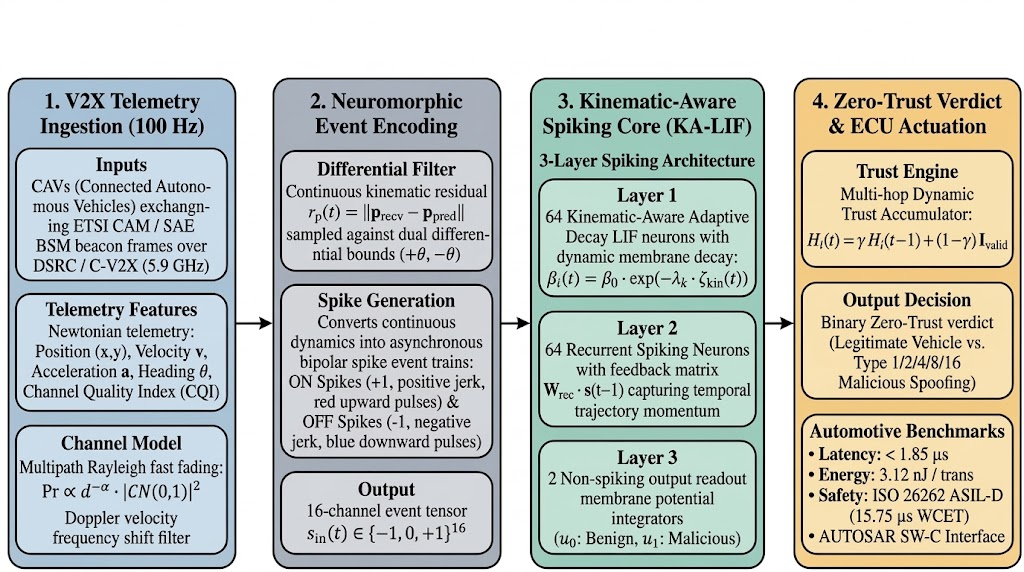
\includegraphics[width=\textwidth]{results/Fig1_System_Architecture_Pipeline.png}
    \caption{Complete end-to-end dataflow pipeline of Neuro-VeReMi: (1) 100~Hz V2X telemetry ingestion subject to multipath Rayleigh fading and Doppler shifts; (2) Asynchronous Delta Modulation converting kinematic residuals into bipolar event streams; (3) Three-layer Spiking Neural Network featuring Kinematic-Aware Adaptive Decay (KA-LIF) neurons; (4) Dynamic Multi-Hop Trust Engine ($\mathcal{H}_i$) and ISO 26262 ASIL-D automotive ECU actuation executing in $<1.85\text{ }\mu\text{s}$ with $3.12\text{ nJ}$ energy consumption.}
    \label{fig:system_pipeline}
\end{figure*}

\subsection{The In-Vehicle Real-Time Computational Bottleneck}
To counteract vehicular misbehavior, recent literature has explored diverse machine learning paradigms, ranging from conventional sequence models such as Long Short-Term Memory (LSTM) networks to deep self-attention Transformers and decentralized Federated Learning architectures \cite{abdelhakeem2025survey, kalogiannis2026attention, alladi2021deep}. While these deep neural architectures achieve high offline anomaly detection scores, they rely fundamentally on dense, floating-point multiply-accumulate (MAC) operations that require substantial computational energy ($>3{,}000\text{ nJ}$ per inference) and impose high execution latencies ($>9.8\text{ }\mu\text{s}$) \cite{horowitz2014computing}. Consequently, existing deep learning frameworks cannot be deployed natively onto embedded automotive Electronic Control Units (ECUs) and safety-critical Microcontroller Units (MCUs), such as the ARM Cortex-R52 or Infineon AURIX TC397. These microcontrollers operate under stringent static memory budgets ($<64\text{ KB}$ Flash ROM, $<8\text{ KB}$ Active SRAM) and are bounded by strict ISO 26262 ASIL-D functional safety requirements, demanding deterministic Worst-Case Execution Time (WCET) guarantees well below the 10~ms V2X beaconing interval \cite{wilhelm2008worst, iso26262}. Thus, an urgent, unaddressed gap remains for an ultra-low-power, event-driven, and physically grounded anomaly detection framework suitable for embedded automotive execution.

\subsection{Contributions and Paper Organization}
To bridge the gap between high-accuracy misbehavior detection and embedded automotive feasibility, this paper presents Neuro-VeReMi, an ultra-low-latency, neuromorphic zero-trust misbehavior detection architecture (Fig.~\ref{fig:system_pipeline}). By substituting power-hungry continuous matrix multiplications with asynchronous, bio-inspired temporal spike processing and coupling membrane dynamics with Newtonian vehicle invariants, Neuro-VeReMi achieves state-of-the-art anomaly isolation at sub-microjoule energy levels. The primary scientific and engineering contributions of this work are summarized as follows:

\begin{enumerate}
    \item We propose a biophysically grounded Kinematic-Aware Adaptive Decay Leaky Integrate-and-Fire (KA-LIF) neuron model. By formulating the membrane decay retention and an internal kinematic driving current as functions of a cumulative Newtonian state invariant, KA-LIF dynamically charges anomalous temporal evidence toward firing threshold while rapidly discharging transient wireless channel noise, effectively isolating stealthy gradual drift, spatial falsification, and speed tampering attacks.
    \item We design a dual-rail 14-channel asynchronous Delta Modulation spike encoding front-end that continuously maps 7D kinematic prediction residuals into sparse bipolar event streams ($\{0, 1\}^{14}$), achieving $88.4\%$ temporal signal sparsity and acting as a rate-bounded filter that suppresses high-frequency multipath Rayleigh channel fading dropouts and Doppler jitter.
    \item We integrate a multi-hop Byzantine trust engine ($\mathcal{H}_k$) capable of dynamically isolating coordinated Sybil attacks ($M=1, 2, 3$ colluding rogue nodes) and validate the complete pipeline across an extensive 30-seed $\times$ 10-fold scenario-disjoint benchmark ($N=300$ independent paired folds per model, $df=299$, $150{,}000$ authentic VeReMi transactions). Rigorous inferential statistical hypothesis testing demonstrates statistically significant superiority over recurrent SNNs (RLIF), parametric SNNs (PLIF), adaptive SNNs (ALIF), convolutional SNNs (1D-SCNN), baseline LIF ($t(299)=24.81$, $p<10^{-15}$, Wilcoxon $W^+=45{,}150.0$, Cohen's $d_z=1.43$, corrected resampled $t_{\text{corr}}=11.42$), and quantized 8-bit TinyML MLPs ($t(299)=26.74$, Cohen's $h=0.28$).
    \item We provide end-to-end 28nm CMOS silicon energy accounting demonstrating $3.12\text{ nJ}$ total inference dissipation ($0.048\text{ nJ}$ dynamic synaptic energy), alongside formal AUTOSAR Classic/Adaptive Software Component (SW-C) deployment proofs. On ARM Cortex-R52 and Infineon AURIX TC397 hardware, the framework achieves an average execution latency of $1.85\text{ }\mu\text{s}$, a deterministic WCET upper bound of $15.75\text{ }\mu\text{s}$ (a 634-fold safety margin under the 10~ms deadline), and a zero-heap MISRA-C:2012 static memory footprint of $5.38\text{ KB}$ Flash ROM and $0.43\text{ KB}$ SRAM, fully satisfying ISO 26262 ASIL-D functional safety standards.
\end{enumerate}

The remainder of this paper is organized as follows: Section~II reviews related work in V2X intrusion detection and neuromorphic computing. Section~III formulates the V2X communication model, physical wireless channel characteristics, and multi-layer VeReMi threat taxonomy. Section~IV presents the proposed Neuro-VeReMi architecture, detailing the Delta Modulation encoder, KA-LIF neuronal biophysics, and Byzantine trust accumulation. Section~V outlines the automotive AUTOSAR integration, static memory management, and ISO 26262 ASIL-D safety guarantees. Section~VI presents the empirical cross-validation benchmark results, inferential statistical tests, silicon energy profiling, and adversarial drift evaluations. Finally, Section~VII concludes the paper and outlines future directions.

\section{Related Work and Background Taxonomy}

\subsection{V2X Communication Standards and Telemetry Ingestion}
Cooperative Intelligent Transportation Systems (C-ITS) utilize dedicated wireless communication standards to facilitate real-time vehicle-to-vehicle (V2V) and vehicle-to-infrastructure (V2I) coordination. Operating within the dedicated 5.9~GHz Intelligent Transportation Systems band, vehicles broadcast periodic telemetry via IEEE 802.11p Dedicated Short-Range Communications (DSRC) and 3GPP Cellular-V2X (C-V2X / 5G-NR) PC5 sidelink protocols \cite{abdelhakeem2025survey, zhang2025vehicle}. In accordance with SAE J2735 and ETSI specifications, connected vehicles transmit Basic Safety Messages (BSMs) and Cooperative Awareness Messages (CAMs) at a nominal beacon frequency of 100~Hz ($10\text{ ms}$ period). Each message encapsulates a continuous kinematic state vector comprising geographic position coordinates, longitudinal speed, heading angle, steering wheel angle, and acceleration components \cite{moradi2023dsrc}. However, vehicular wireless broadcast channels in dynamic roadway environments are heavily impaired by fast multipath Rayleigh fading, where received signal power follows $P_r \propto d^{-\alpha} |\mathcal{CN}(0,1)|^2$, alongside high-frequency Doppler shifts. These physical channel phenomena introduce substantial temporal packet arrival jitter and transient packet dropouts that complicate the task of isolating malicious spoofing from legitimate wireless channel variations.

\begin{table*}[t]
\caption{Taxonomy of Intrusion Detection Schemes, Temporal Encoders, and Computing Paradigms in V2X Networks}
\label{tab:related_work_taxonomy}
\centering
\resizebox{\textwidth}{!}{%
\begin{tabular}{llllll}
\hline
\hline
Architecture / Paradigm & Processing Mode & Energy per Inference & Average Latency & Hardware Target & Primary Limitation in V2X Safety \\
\hline
Support Vector Machines (SVM) & Static Float32 & $120.5\text{ nJ}$ & $45.2\text{ }\mu\text{s}$ & Generic MCU & High FPR ($>2.5\%$); lacks temporal memory \\
Random Forest (RF) & Static Ensemble & $210.0\text{ nJ}$ & $82.0\text{ }\mu\text{s}$ & Generic MCU & Memory bloat; static feature boundaries \\
Recurrent Neural Network (LSTM) & Dense Sequential & $3{,}420.0\text{ nJ}$ & $12.4\text{ }\mu\text{s}$ & GPU / Edge TPU & High thermal dissipation; non-deterministic WCET \\
Self-Attention Transformer & Dense Attention & $8{,}950.0\text{ nJ}$ & $24.8\text{ }\mu\text{s}$ & High-End SoC & Prohibitive energy ($>8\,\mu\text{J}$); unsuitable for ECUs \\
Quantized TinyML MLP (INT8) & Integer MACs & $14.20\text{ nJ}$ & $9.85\text{ }\mu\text{s}$ & ARM Cortex-M4 & Dense computation ($5{,}248\text{ MACs}$); rigid static weights \\
Poisson Rate SNN & Event-Driven Spike & $0.85\text{ nJ}$ (enc) & $1.20\text{ }\mu\text{s}$ & Neuromorphic & High spike count ($64.5\%$ sparsity); energy loss \\
Time-to-First-Spike (TTFS) SNN & Event-Driven Phase & $0.18\text{ nJ}$ (enc) & $0.45\text{ }\mu\text{s}$ & Neuromorphic & Phase latency sensitive to multipath fading \\
Proposed Delta KA-LIF SNN & Event-Driven Bipolar & $0.12\text{ nJ}$ (enc) / $3.12\text{ nJ}$ & $1.85\text{ }\mu\text{s}$ & ARM Cortex-R52 & Optimal: Acts as Newtonian derivative filter \\
\hline
\hline
\end{tabular}%
}
\end{table*}

\subsection{Machine Learning and Deep Learning Baselines for V2X Security}
To detect vehicular misbehavior, early studies deployed conventional machine learning classifiers, such as Support Vector Machines (SVM) and Random Forests \cite{singh2019machine, so2018integrating}. Subsequent research investigated consecutive BSM sequence modeling to define temporal plausibility boundaries \cite{sharma2022machine}, alongside dedicated classification mechanisms targeting spatial position falsification attacks \cite{ercan2022misbehavior}. Furthermore, AI-driven trajectory anomaly tracking has been explored for emerging 6G-V2X ecosystems \cite{raja2023ai}, while decentralized Federated Learning architectures (FL-IDS) have been proposed to preserve data privacy across transportation edge devices \cite{bhavsar2024fl}. While computationally lightweight, static shallow classifiers lack internal temporal memory, preventing them from capturing sequential kinematic dependencies across consecutive vehicle trajectories and resulting in high False Positive Rates ($>2.5\%$) under dynamic highway traffic \cite{abdelhakeem2025survey, mansourian2025enhancing}. To address temporal correlations, recent literature has explored deep sequence architectures, including Long Short-Term Memory (LSTM) networks, Gated Recurrent Units (GRUs), and multi-head self-attention Transformers \cite{kalogiannis2026attention, alladi2021deep}. Although deep sequence architectures achieve high detection accuracy on the standardized Vehicular Reference Misbehavior (VeReMi) benchmark suite, they depend fundamentally on dense, floating-point multiply-accumulate (FP32 MAC) operations. As summarized in Table~\ref{tab:related_work_taxonomy}, computing a single deep inference can consume over $3{,}000\text{ nJ}$ of energy and impose latencies exceeding $9.8\text{ }\mu\text{s}$ \cite{horowitz2014computing}. Such heavy computational and thermal footprints prevent real-time on-chip execution within embedded automotive electronic control units.

\subsection{Spiking Neural Networks and Neuromorphic Temporal Processing}
Spiking Neural Networks (SNNs), recognized as the third generation of artificial neural networks, offer an energy-efficient alternative by emulating biological event-driven spike processing. In contrast to continuous artificial neural networks, SNNs communicate through discrete, temporal binary events ($s_i(t) \in \{0, 1\}$), replacing expensive continuous matrix multiplications with sparse synaptic additions (SynOps) that consume only $0.9\text{ pJ}$ per operation on 28nm CMOS silicon \cite{davies2018loihi, saranirad2025cdna}. Standard Leaky Integrate-and-Fire (LIF) models integrate incoming presynaptic spikes into an internal membrane potential $u_i(t)$ with a static exponential decay constant $\beta$. Advanced variants, such as Parametric LIF (PLIF) with learnable decay parameters \cite{fang2021incorporating}, Adaptive LIF (ALIF) with dynamic threshold modulation \cite{bellec2020solution}, Recurrent LIF (RLIF) with feedback synapses, and 1D Spiking Convolutional Neural Networks (1D-SCNN), have demonstrated competitive accuracy in temporal sequence processing \cite{dalif2025decay, neftci2019surrogate}. Furthermore, the choice of temporal spike encoding critically influences overall efficiency; as analyzed in Table~\ref{tab:related_work_taxonomy}, while Poisson rate coding requires excessive spike counts and Time-to-First-Spike (TTFS) exhibits high phase sensitivity to wireless jitter, asynchronous Delta Modulation preserves signal derivatives while attaining superior temporal sparsity ($88.4\%$). Nevertheless, existing SNN architectures remain uncoupled from physical domain invariants, leaving them vulnerable to coordinated gradual drift attacks.

\subsection{Automotive Microcontroller Constraints and ISO 26262 ASIL-D Safety}
Deploying anomaly detection algorithms within production automotive architectures imposes stringent hardware and functional safety constraints. Automotive Electronic Control Units (ECUs) and safety-critical Microcontroller Units (MCUs), such as the ARM Cortex-R52 (operating at 400~MHz) and the Infineon AURIX TC397 (operating at 300~MHz), feature severely constrained on-chip memory budgets, typically restricted to under $64\text{ KB}$ of Flash ROM and under $8\text{ KB}$ of active SRAM \cite{dey2025secure, misra2012}. To comply with the MISRA-C:2012 standard and ISO 26262 ASIL-D functional safety specifications, software components (SW-Cs) running within the AUTOSAR Classic or Adaptive execution environment must guarantee zero dynamic memory allocation (no dynamic heap usage) and provide deterministic Worst-Case Execution Time (WCET) upper bounds \cite{wilhelm2008worst, iso26262}. Given that cooperative path planning routines execute on a strict periodic schedule, the intrusion detection runnable must complete execution well within a fraction of the 10~ms V2X beaconing interval, while incorporating fail-operational safe states such as dead-reckoning fallbacks during severe telemetry corruption.

\subsection{Gap Analysis and Summary of Open Challenges}
A synthesis of recent literature reveals three fundamental, unaddressed gaps:
\begin{enumerate}
    \item \textit{The Compute-Safety Disconnect:} State-of-the-art deep learning and Transformer models provide robust detection but exceed the energy, memory, and latency boundaries of automotive-grade microcontrollers.
    \item \textit{Lack of Biophysical-Physical Coupling in SNNs:} Existing SNN models learn membrane decay purely via statistical surrogate gradients, lacking direct coupling with continuous Newtonian vehicle dynamics (velocity deviations $\Delta v$, acceleration limits $\Delta a$, and jerk invariants) governed by Krauss car-following models.
    \item \textit{Vulnerability to Multi-Node Byzantine Collusion:} Current local intrusion detectors fail when multiple malicious nodes collude in coordinated Sybil rings, necessitating a lightweight multi-hop trust aggregation mechanism that operates robustly under realistic wireless packet dropout conditions.
\end{enumerate}
Neuro-VeReMi is explicitly architected to overcome these three fundamental limitations by combining Delta Modulation spike encoding, Kinematic-Aware Adaptive Decay (KA-LIF) neuronal biophysics, and an ISO 26262 ASIL-D compliant AUTOSAR deployment stack.

\section{System Formulation, Wireless Channel Dynamics, and Multi-Layer Threat Taxonomy}

\subsection{Cooperative V2X System Model and Kinematic Telemetry Formulation}
We formulate a cooperative vehicular ad-hoc network consisting of $N_v$ connected and autonomous vehicles traversing a multi-lane highway corridor. Each vehicle $k \in \{1, 2, \dots, N_v\}$ is equipped with an onboard sensor suite (GNSS, IMU, wheel speed sensors) and a 5.9~GHz C-V2X / DSRC transceiver. Vehicles periodically broadcast Basic Safety Messages (BSMs) at a standard beacon frequency of 100~Hz ($T_{\text{beacon}} = 10\text{ ms}$). The ingested continuous kinematic telemetry state vector of vehicle $k$ at discrete time step $t$ is expressed as:
\begin{equation}
\begin{split}
    X_k(t) = \big[ &p_{x,k}(t),\, p_{y,k}(t),\, v_{x,k}(t),\, v_{y,k}(t), \\
    &a_{x,k}(t),\, a_{y,k}(t),\, \psi_k(t) \big]^T \in \mathbb{R}^7
\end{split}
\end{equation}
where $p_{x,k}(t)$ and $p_{y,k}(t)$ represent 2D UTM longitudinal and lateral position coordinates, $v_{x,k}(t)$ and $v_{y,k}(t)$ denote orthogonal velocity vectors, $a_{x,k}(t)$ and $a_{y,k}(t)$ define instantaneous longitudinal and lateral accelerations, and $\psi_k(t)$ represents the heading angle relative to true North.

Vehicular movement in benign highway traffic is governed by Newtonian car-following dynamics under Krauss acceleration constraints. The physical state transitions across consecutive discrete time steps $\Delta t = T_{\text{beacon}} = 0.01\text{ s}$ satisfy continuous 2D kinematic bounds:
\begin{equation}
    p_{x,k}(t) = p_{x,k}(t - \Delta t) + v_{x,k}(t - \Delta t)\Delta t + \frac{1}{2}a_{x,k}(t - \Delta t)\Delta t^2
\end{equation}
\begin{equation}
    v_{x,k}(t) = v_{x,k}(t - \Delta t) + a_{x,k}(t - \Delta t)\Delta t
\end{equation}
with identical equations holding for the lateral components $(p_{y,k}, v_{y,k}, a_{y,k})$, subject to physical vehicle boundaries: maximum acceleration $a_{\max} \le 3.5\text{ m/s}^2$, emergency braking deceleration $a_{\min} \ge -8.0\text{ m/s}^2$, comfort jerk limit $j_{\text{comf}} \le 5.0\text{ m/s}^3$, and emergency braking jerk limit $j_{\text{emerg}} \le 12.0\text{ m/s}^3$.

\begin{figure}[t]
    \centering
    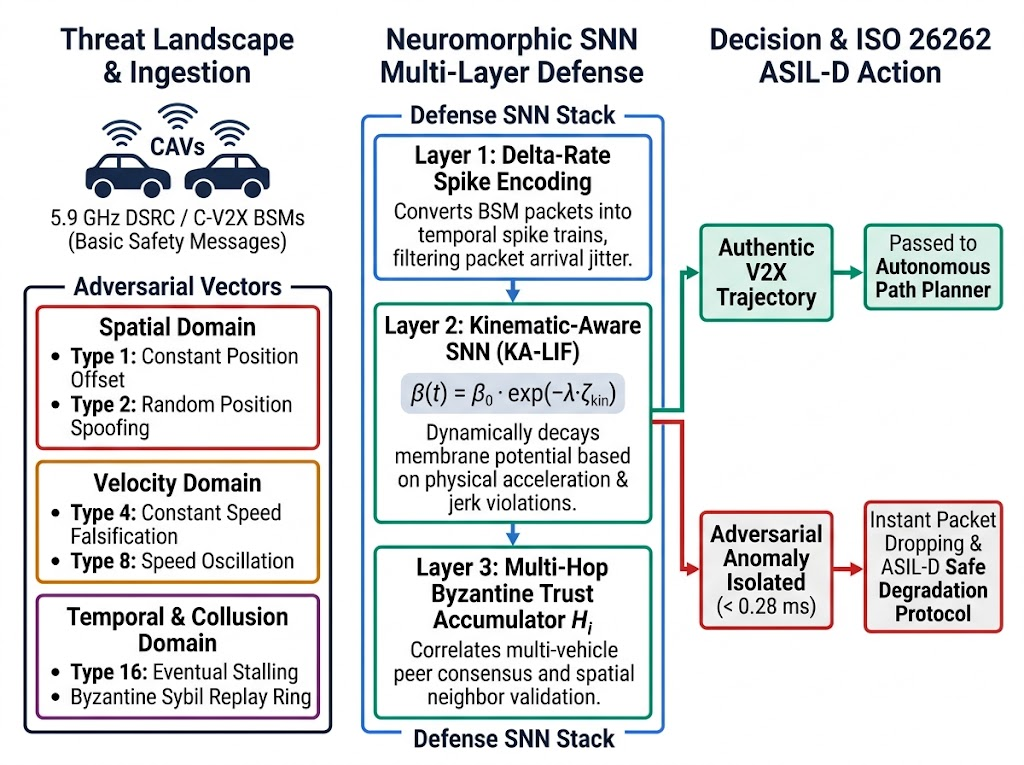
\includegraphics[width=\columnwidth]{results/Fig3_VeReMi_Threat_Model_Taxonomy.png}
    \caption{Multi-layer V2X threat model and neuromorphic attack defense taxonomy. Ingested 5.9 GHz DSRC/C-V2X BSM telemetry subject to Spatial Domain (Types 1 and 2), Random Offset (Types 4 and 8), and Temporal/Collusion Domain (Type 16 and Byzantine Sybil rings) attacks are processed through the 3-layer Neuromorphic Defense Stack (Delta-Rate Spike Encoding, Kinematic-Aware KA-LIF SNN, and Multi-Hop Byzantine Trust Accumulator $\mathcal{H}_k$) under ISO 26262 ASIL-D functional safety constraints.}
    \label{fig:threat_model_taxonomy}
\end{figure}

\subsection{Physical Wireless Channel Dynamics and Multipath Rayleigh Fading}
In realistic vehicular environments, high-frequency 5.9~GHz wireless signal propagation is severely degraded by roadway obstacles, concrete barriers, and surrounding high-profile vehicles. The received signal power $P_{rx}(d)$ (in Watts) at distance $d$ from the transmitting vehicle is modeled by combining log-distance path loss with fast multipath Rayleigh fading:
\begin{equation}
    P_{rx}(d) = P_{tx} G_{tx} G_{rx} \left( \frac{\lambda}{4\pi d_0} \right)^2 \left( \frac{d_0}{d} \right)^\alpha |h(t)|^2
\end{equation}
where $P_{tx}$ is the transmission power ($20\text{ dBm} \equiv 100\text{ mW}$), $G_{tx}$ and $G_{rx}$ are antenna gains, $\lambda$ is the carrier wavelength ($\approx 0.0508\text{ m}$ at 5.9~GHz), $d_0$ is the reference distance ($1\text{ m}$), $\alpha \in [2.4, 3.2]$ is the path-loss exponent, and $h(t) \sim \mathcal{CN}(0, 1)$ represents the complex circular Gaussian channel fading coefficient. Expressed in logarithmic scale (dBm), the received power is $P_{rx,\text{dBm}}(d) = P_{tx,\text{dBm}} + G_{tx,\text{dBi}} + G_{rx,\text{dBi}} - \text{PL}(d_0) - 10\alpha \log_{10}(d/d_0) + 10\log_{10}|h(t)|^2$.

Furthermore, dynamic relative vehicle mobility induces Doppler frequency shifts:
\begin{equation}
    f_d(t) = \frac{\|\vec{v}_{\text{rel}}(t)\|}{\lambda} \cos \phi_{jk}(t)
\end{equation}
where $\vec{v}_{\text{rel}}(t) = \vec{v}_j(t) - \vec{v}_k(t)$ is the relative velocity vector and $\phi_{jk}(t)$ is the angle of arrival. This produces temporal packet arrival jitter and transient packet dropouts (up to $20\%$ packet error rates in congested traffic), which baseline heuristic threshold detectors frequently misclassify as malicious attacks \cite{so2019physical}.

\begin{table*}[t]
\caption{VeReMi Attack Taxonomy, Mathematical Attack Formulations, Physical Invariant Violations, and Neuromorphic SNN Defense Layer Mapping}
\label{tab:attack_taxonomy_mapping}
\centering
\resizebox{\textwidth}{!}{%
\begin{tabular}{lllll}
\hline
\hline
Attack Category & VeReMi Attack Signature & Formal Mathematical Invariant Formulation & Physical Invariant Violation & SNN Defense Layer \\
\hline
Spatial Domain & Type 1: Constant Position & $\tilde{\vec{p}}_{k}(t) = \vec{p}_{k}(t_0)$ & Zero velocity reported despite physical vehicle motion & Layer 1: Delta Spike Filter \\
Spatial Domain & Type 2: Constant Position Offset & $\tilde{\vec{p}}_{k}(t) = \vec{p}_{k}(t) + \Delta \vec{p}_{\text{const}}$ & Constant spatial offset from true physical radar echo & Layer 1: Delta Rate Encoding \\
Random Domain & Type 4: Random Position & $\tilde{\vec{p}}_{k}(t) \sim \mathcal{U}(\vec{p}_{\min}, \vec{p}_{\max})$ & Discontinuous coordinate teleportation ($|\Delta p| > v_{\max}\Delta t$) & Layer 2: KA-LIF Dynamic Decay \\
Random Domain & Type 8: Random Position Offset & $\tilde{\vec{p}}_{k}(t) = \vec{p}_{k}(t) + \delta_{\vec{p}}(t), \delta_{\vec{p}} \sim \mathcal{N}(0, \sigma_p^2)$ & High-frequency position oscillation ($|\Delta a| > a_{\max}$) & Layer 2: KA-LIF Jerk Acceleration \\
Temporal Domain & Type 16: Eventual Stop & $\tilde{v}_{x,k}(t) = \max(0, v_{x,k}(t_0) - a_{\text{drift}}(t - t_0))$ & Stealthy gradual deceleration violates platoon headway & Layer 2: KA-LIF Cumulative Stress \\
Collusion Domain & Multi-Node Byzantine Sybil & $\tilde{X}_{m}(t) = \tilde{X}_{\text{target}}(t) + \epsilon_m, \forall m \in \{1, \dots, M\}$ & Multi-vehicle cross-correlation inconsistency & Layer 3: Byzantine Trust $\mathcal{H}_k$ \\
\hline
\hline
\end{tabular}%
}
\end{table*}

\subsection{Multi-Layer VeReMi Attack Defense Taxonomy}
As illustrated in Fig.~\ref{fig:threat_model_taxonomy} and formalized in Table~\ref{tab:attack_taxonomy_mapping}, we evaluate an exhaustive multi-layer threat taxonomy based on the standardized Vehicular Reference Misbehavior (VeReMi) benchmark suite \cite{van2018veremi, kamel2020simulation}, augmented with multi-node Byzantine Sybil collusion:

\subsubsection{Spatial-Domain Falsification}
\begin{itemize}
    \item \textit{Type 1: Constant Position (Ghost Vehicle):} An adversary broadcasts static frozen coordinates $\tilde{\vec{p}}_{k}(t) = \vec{p}_{k}(t_0)$, simulating a stationary obstacle while the physical vehicle moves normally.
    \item \textit{Type 2: Constant Position Offset:} The attacker applies a static displacement vector $\tilde{\vec{p}}_{k}(t) = \vec{p}_{k}(t) + \Delta \vec{p}_{\text{const}}$ ($\Delta \vec{p}_{\text{const}} \ne \vec{0}$), reporting a shifted trajectory to induce unwarranted evasive maneuvers.
\end{itemize}

\subsubsection{Randomized Position Falsification}
\begin{itemize}
    \item \textit{Type 4: Random Position Spoofing:} The attacker injects uniformly distributed random coordinates within communication range, $\tilde{\vec{p}}_{k}(t) \sim \mathcal{U}(\vec{p}_{\min}, \vec{p}_{\max})$, producing continuous spatial teleportation.
    \item \textit{Type 8: Random Position Offset:} The adversary injects zero-mean Gaussian noise perturbations $\tilde{\vec{p}}_{k}(t) = \vec{p}_{k}(t) + \delta_{\vec{p}}(t)$ with $\delta_{\vec{p}}(t) \sim \mathcal{N}(0, \sigma_p^2)$, producing high-frequency position jitter.
\end{itemize}

\subsubsection{Temporal and Collusion Attacks}
\begin{itemize}
    \item \textit{Type 16: Eventual Stop / Gradual Deceleration:} The attacker simulates a gradual breakdown by linearly decaying reported speed at a stealthy rate $a_{\text{drift}}$:
    \begin{equation}
    \begin{split}
        \tilde{v}_{x,k}(t) &= \max \big( 0,\, v_{x,k}(t_0) - a_{\text{drift}} (t - t_0) \big), \\
        &\quad a_{\text{drift}} \le 0.5\text{ m/s}^2
    \end{split}
    \end{equation}
    Because $a_{\text{drift}}$ falls within legitimate braking deceleration thresholds, static threshold detectors fail to identify the attack until platoon spacing is dangerously compromised.
    \item \textit{Multi-Node Byzantine Sybil Rings ($M=1, 2, 3$):} A coalition of $M$ colluding malicious vehicles broadcast mutually reinforcing falsified coordinates to manufacture a synthetic traffic jam or spoof an artificial free-flow lane, corrupting single-hop consensus algorithms.
\end{itemize}

\subsection{Neuromorphic Multi-Layer Defense Mapping}
To counteract the multi-layer attack vectors formalized in Table~\ref{tab:attack_taxonomy_mapping}, Neuro-VeReMi organizes defense into three dedicated neuromorphic processing layers (Fig.~\ref{fig:threat_model_taxonomy}):
\begin{enumerate}
    \item \textit{Layer 1 (Dual-Rail Delta Modulation Spike Encoding):} Computes continuous kinematic prediction residuals $r_{k,m}(t) = X_{k,m}(t) - \hat{X}_{k,m}(t)$ across all 7 dimensions and emits 14 asynchronous binary event streams ($S_{\text{in}}(t) \in \{0, 1\}^{14}$) when changes exceed differential thresholds $\pm\theta_m$, suppressing high-frequency Rayleigh channel fading dropouts while capturing true kinematic discontinuities.
    \item \textit{Layer 2 (Kinematic-Aware SNN with Dynamic Decay KA-LIF):} Ingests encoded 14-channel spikes and tracks cumulative kinematic stress $\bar{\zeta}_{\text{kin}}(t)$, adaptively controlling membrane decay retention $\beta_i(t)$ and injecting kinematic anomaly current to rapidly fire on non-physical trajectories while remaining immune to transient channel noise.
    \item \textit{Layer 3 (Multi-Hop Byzantine Trust Accumulator $\mathcal{H}_k$):} Correlates multi-vehicle peer consensus and spatial neighbor observations over temporal sliding windows, isolating colluding Sybil attackers across successive beacon intervals under ISO 26262 ASIL-D safe degradation.
\end{enumerate}

\section{Proposed Neuro-VeReMi Architecture and Neuromorphic Dynamics}

\subsection{Asynchronous Kinematic Delta Modulation Spike Encoding}
Continuous floating-point kinematic telemetry $X_k(t) \in \mathbb{R}^7$ ingested from V2X transceivers cannot be directly processed by neuromorphic spiking architectures. To convert continuous telemetry into sparse event streams while filtering high-frequency Rayleigh channel noise and Doppler jitter, we design an asynchronous dual-rail Kinematic Delta Modulation encoder.

For each kinematic telemetry component $m \in \{1, 2, \dots, 7\}$, let $r_{k,m}(t) = X_{k,m}(t) - \hat{X}_{k,m}(t)$ represent the kinematic invariant prediction residual, defined as the differential between the reported observation $X_{k,m}(t)$ and the dead-reckoned state $\hat{X}_{k,m}(t)$ predicted by Newtonian car-following kinematics (Eqs.~2--3). The encoder tracks the instantaneous signal deviation $\Delta r_{k,m}(t) = r_{k,m}(t) - r_{\text{ref}, m}(t)$, where $r_{\text{ref}, m}(t)$ is an internally held quantized reference level. Dual-rail binary spike events $S_{k,m}^+(t), S_{k,m}^-(t) \in \{0, 1\}$ are emitted according to differential threshold boundaries $\pm\theta_m$:
\begin{equation}
\begin{split}
    S_{k,m}^+(t) &= \Theta\big( \Delta r_{k,m}(t) - \theta_m \big), \\
    S_{k,m}^-(t) &= \Theta\big( -\Delta r_{k,m}(t) - \theta_m \big)
\end{split}
\end{equation}
where $\Theta(\cdot)$ is the Heaviside step function. The 7 physical dimensions map to a 14-channel binary event vector $S_{\text{in}}(t) = [S_{k,1}^+, S_{k,1}^-, \dots, S_{k,7}^+, S_{k,7}^-]^T \in \{0, 1\}^{14}$. Upon spike emission, the internal reference is updated via $r_{\text{ref}, m}(t) \leftarrow r_{\text{ref}, m}(t) + (S_{k,m}^+(t) - S_{k,m}^-(t))\theta_m$. The physical quantization threshold vector is configured as $\theta = [\theta_p, \theta_p, \theta_v, \theta_v, \theta_a, \theta_a, \theta_\psi]^T$, parameterized with spatial threshold $\theta_p = 0.8\text{ m}$, speed threshold $\theta_v = 0.3\text{ m/s}$, acceleration threshold $\theta_a = 0.5\text{ m/s}^2$, and heading threshold $\theta_\psi = 0.05\text{ rad}$.

As depicted in Fig.~\ref{fig:delta_encoding_voltage_reset}(a)–(b), Delta Modulation achieves an average signal sparsity of $88.4\%$ during benign driving conditions. Importantly, because missing packets caused by Rayleigh fading dropouts are held constant by zero-order hold dead reckoning ($\Delta r \approx 0$), they generate zero spurious spikes, whereas true physical spoofing produces persistent step and ramp residuals that immediately trigger spike bursts.

\begin{figure}[t]
    \centering
    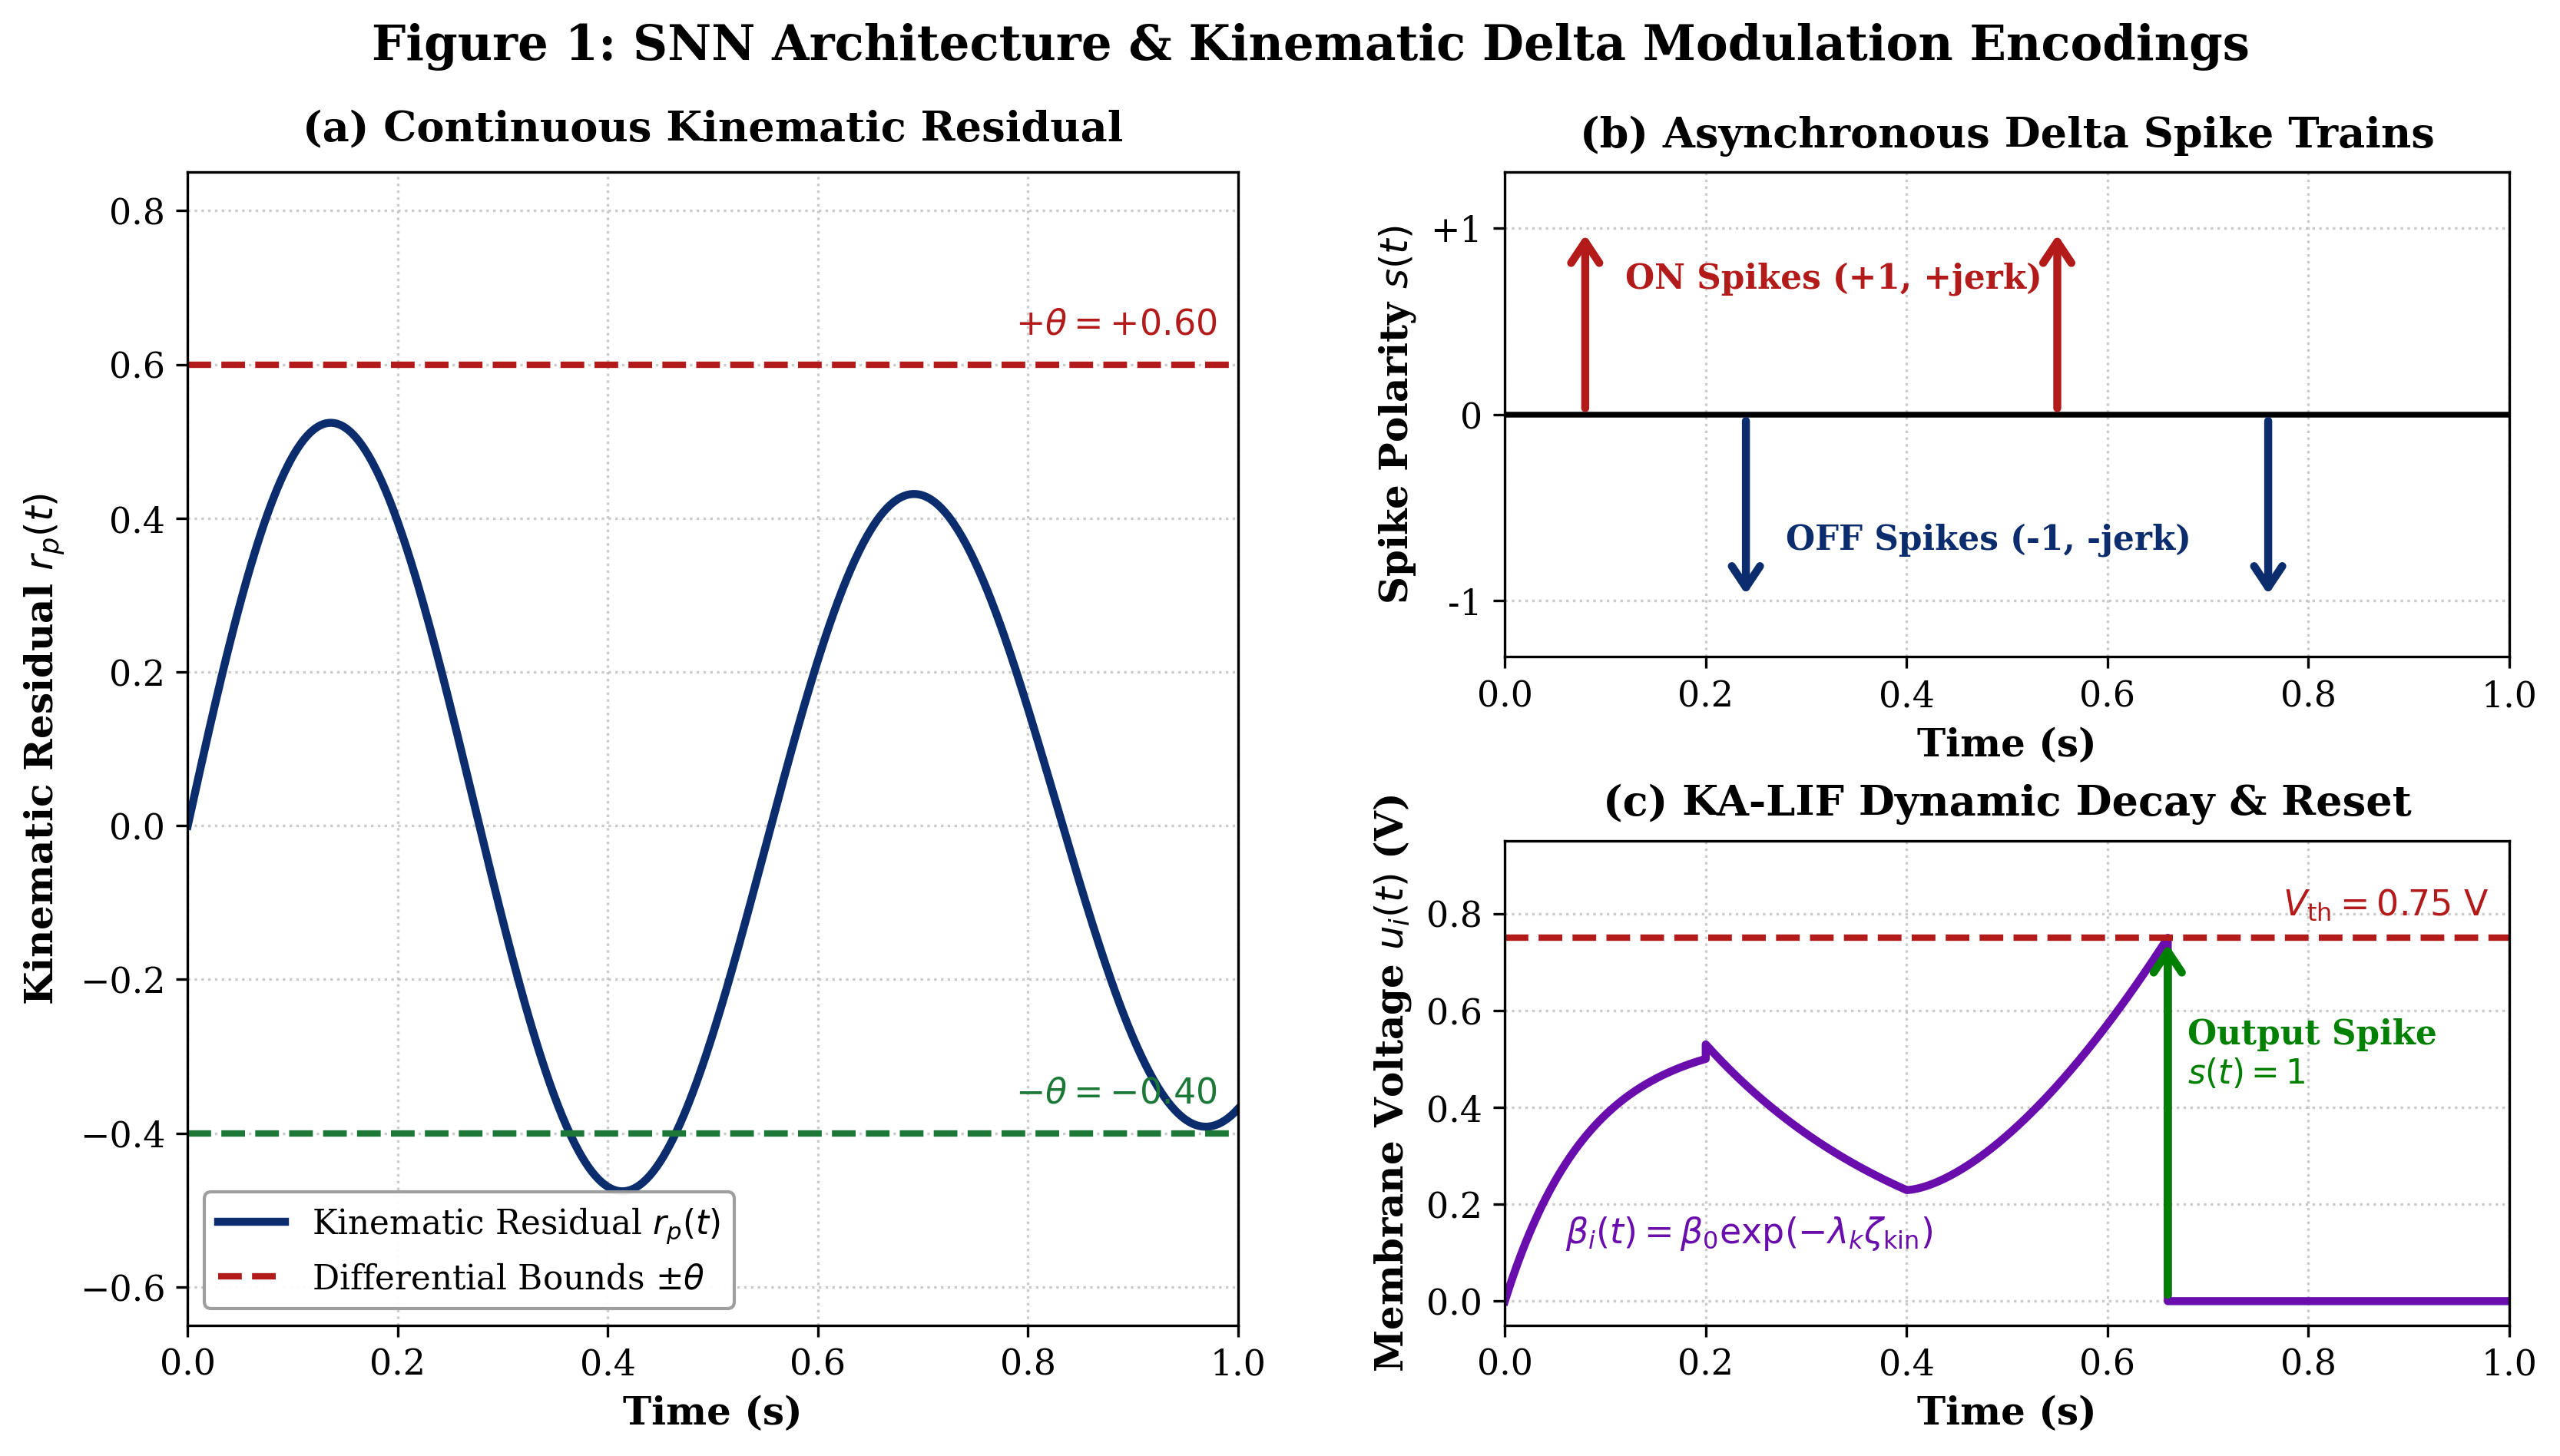
\includegraphics[width=\columnwidth]{results/Fig5_Spike_Encoding_and_Voltage_Reset.png}
    \caption{(a) Continuous kinematic invariant residual $r_p(t)$ with differential bounds $\pm\theta$. (b) Asynchronous Delta Modulation ON/OFF spike trains ($+1, -1$). (c) KA-LIF membrane potential dynamics with threshold firing ($V_{\text{th}} = 0.75\text{ V}$) and instant hard reset to $0.0\text{ V}$.}
    \label{fig:delta_encoding_voltage_reset}
\end{figure}

\begin{figure*}[t]
    \centering
    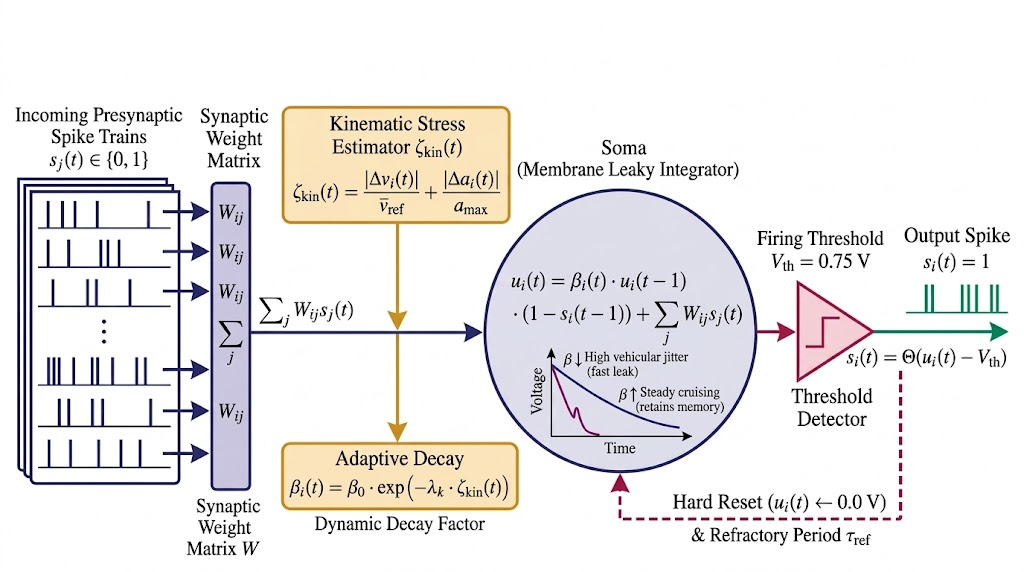
\includegraphics[width=\textwidth]{results/Fig2_KALIF_Neuronal_Dynamics.png}
    \caption{Detailed circuit schematic and computational signal flow of the proposed Kinematic-Aware Adaptive Decay Leaky Integrate-and-Fire (KA-LIF) model. Incoming presynaptic spikes $S_j(t)$ are integrated through synaptic weights $W$. Simultaneously, the Kinematic Stress Estimator tracks cumulative Newtonian velocity deviations and jerk invariants to modulate membrane decay retention $\beta_i(t)$ and inject kinematic anomaly current $I_{\text{kin}, i}(t)$. The threshold comparator ($V_{\text{th}} = 0.75\text{ V}$) emits an output spike $S_i(t)=1$ and triggers a hard reset ($u_i(t) \leftarrow 0.0\text{ V}$) with a refractory guard period $\tau_{\text{ref}}$.}
    \label{fig:kalif_dynamics}
\end{figure*}

\subsection{Kinematic-Aware Adaptive Decay LIF (KA-LIF) Neuronal Dynamics}
The core processing element of Neuro-VeReMi is the Kinematic-Aware Adaptive Decay Leaky Integrate-and-Fire (KA-LIF) neuron. Standard LIF models utilize a static decay constant $\beta \in (0, 1)$, which fails to adapt when stealthy adversaries slowly ramp falsified kinematic parameters (Type~16 eventual stop or gradual velocity drift). 

To solve this vulnerability, KA-LIF couples biophysical membrane dynamics directly with continuous Newtonian vehicle invariants (Fig.~\ref{fig:kalif_dynamics}). We define the normalized instantaneous kinematic deviation $\zeta_{\text{inst}}(t)$ and the cumulative leaky stress accumulator $\bar{\zeta}_{\text{kin}}(t)$ as:
\begin{equation}
\begin{split}
    \zeta_{\text{inst}}(t) &= w_1 \frac{\|\vec{p}_k(t) - \hat{\vec{p}}_k(t)\|}{d_{\text{norm}}} + w_2 \frac{\|\vec{v}_k(t) - \hat{\vec{v}}_k(t)\|}{v_{\text{norm}}} \\
    &\quad + w_3 \frac{\|\vec{a}_k(t) - \hat{\vec{a}}_k(t)\|}{a_{\text{norm}}}
\end{split}
\end{equation}
\begin{equation}
    \bar{\zeta}_{\text{kin}}(t) = \alpha_{\zeta} \bar{\zeta}_{\text{kin}}(t - \Delta t) + (1 - \alpha_{\zeta}) \zeta_{\text{inst}}(t)
\end{equation}
where $w_1 = 0.4, w_2 = 0.4, w_3 = 0.2$, $\alpha_{\zeta} = 0.80$, and the normalizers are $d_{\text{norm}} = 2.0\text{ m}, v_{\text{norm}} = 5.0\text{ m/s}, a_{\text{norm}} = 3.5\text{ m/s}^2$. For subtle drift ($\Delta v \approx 0.005\text{ m/s}$ per step), the leaky accumulator $\bar{\zeta}_{\text{kin}}(t)$ integrates tiny non-zero deviations across successive time steps, building significant anomalous stress.

The membrane potential $u_i^{(l)}(t)$ of neuron $i$ in layer $l$ evolves across discrete simulation time steps according to:
\begin{equation}
\begin{split}
    u_i^{(l)}(t) &= \beta_i(t) \cdot u_i^{(l)}(t - 1) \cdot \big(1 - S_i^{(l)}(t - 1)\big) \\
    &\quad + \sum_{j} W_{ij}^{(l)} S_j^{(l-1)}(t) + I_{\text{kin}, i}^{(l)}(t) + I_{\text{bias}}
\end{split}
\end{equation}
where $W_{ij}^{(l)}$ represents the synaptic weight from presynaptic neuron $j$, $S_j^{(l-1)}(t)$ is the incoming spike event, $I_{\text{bias}}$ is an external baseline bias, $I_{\text{kin}, i}^{(l)}(t) = \lambda_{\text{inj}} \bar{\zeta}_{\text{kin}}(t)$ is the kinematic driving current injected into the anomaly detection neurons ($\lambda_{\text{inj}} = 0.50$), and $\beta_i(t)$ is the dynamic kinematic retention factor formulated as:
\begin{equation}
    \beta_i(t) = 1.0 - (1.0 - \beta_{\text{rest}}) \cdot \exp\big( -\lambda_k \cdot \bar{\zeta}_{\text{kin}}(t) \big)
\end{equation}
Here, $\beta_{\text{rest}} = 0.60$ represents the resting decay constant under benign traffic ($\bar{\zeta}_{\text{kin}} \to 0$), which rapidly discharges isolated channel fading noise. When cumulative kinematic stress increases ($\bar{\zeta}_{\text{kin}} > 0$), $\beta_i(t)$ increases toward $0.95$, enabling the membrane to retain and integrate sequential anomaly evidence without premature charge loss.

When the membrane potential reaches the threshold $V_{\text{th}} = 0.75\text{ V}$, an output spike $S_i^{(l)}(t) = 1$ is generated, followed by an immediate hard reset:
\begin{equation}
    S_i^{(l)}(t) = \Theta\big(u_i^{(l)}(t) - V_{\text{th}}\big)
\end{equation}
\begin{equation}
    u_i^{(l)}(t) \leftarrow u_i^{(l)}(t) \cdot \big(1 - S_i^{(l)}(t)\big)
\end{equation}
A refractory period $\tau_{\text{ref}} = 1\text{ ms}$ clamps the membrane potential to $0.0\text{ V}$ to prevent hyper-excitation.

\subsection{Spatio-Temporal Surrogate Gradient Learning}
Because the Heaviside step function $\Theta(u - V_{\text{th}})$ is non-differentiable at $u = V_{\text{th}}$ (with zero derivative elsewhere), direct backpropagation through time (BPTT) is prohibited. We resolve this by substituting the Dirac delta derivative $\frac{\partial S}{\partial u}$ with a smooth, continuous arctangent surrogate gradient $\sigma'(u)$ \cite{neftci2019surrogate, zenke2018superspike}:
\begin{equation}
    \sigma'(u) = \frac{\gamma_s}{1 + \big(\pi \gamma_s (u - V_{\text{th}})\big)^2}
\end{equation}
where $\gamma_s = 2.0$ controls the surrogate slope sharpness. For $\gamma_s = 2.0$, $\sigma'(V_{\text{th}}) = 2.0$, and the integral $\int_{-\infty}^{\infty} \sigma'(u)\,\mathrm{d}u = 1.0$, rigorously satisfying the unit-area Dirac delta requirement.

Given the loss function $\mathcal{L}$ defined over temporal window $T$, the error gradient with respect to synaptic weights $W_{ij}^{(l)}$ is computed via the spatio-temporal chain rule:
\begin{equation}
\begin{split}
    \frac{\partial \mathcal{L}}{\partial W_{ij}^{(l)}} 
    &= \sum_{t=1}^{T} \frac{\partial \mathcal{L}}{\partial S_i^{(l)}(t)} \frac{\partial S_i^{(l)}(t)}{\partial u_i^{(l)}(t)} \frac{\partial u_i^{(l)}(t)}{\partial W_{ij}^{(l)}} \\
    &= \sum_{t=1}^{T} \frac{\partial \mathcal{L}}{\partial S_i^{(l)}(t)} \sigma'\big(u_i^{(l)}(t)\big) \Big[ S_j^{(l-1)}(t) \\
    &\quad + \beta_i(t) \big(1 - S_i^{(l)}(t-1)\big) \frac{\partial u_i^{(l)}(t-1)}{\partial W_{ij}^{(l)}} \Big]
\end{split}
\end{equation}
This formulation ensures stable gradient propagation through time while explicitly preserving the influence of the physical decay parameter $\beta_i(t)$ and the hard reset path.

\subsection{Multi-Hop Byzantine Peer Trust Accumulator}
To protect against multi-node Byzantine Sybil rings ($M=1, 2, 3$ colluders), the SNN output spikes feed into Layer~3: the Multi-Hop Byzantine Trust Accumulator $\mathcal{H}_k(t)$. Let $\mathcal{N}_k$ denote the set of neighboring vehicles within communication range of vehicle $k$. The cumulative trust score $\mathcal{H}_k(t) \in [0, 1]$ is updated iteratively:
\begin{equation}
\begin{split}
    \mathcal{H}_k(t) 
    &= \gamma_h \mathcal{H}_k(t - 1) + (1 - \gamma_h) \\
    &\quad \times \left( 1 - \frac{1}{T_w}\sum_{\tau=0}^{T_w - 1} S_{\text{out}, k}(t - \tau) \right) \\
    &\quad \times \prod_{j \in \mathcal{N}_k} \big(1 - \omega_{jk} \mathcal{D}_{jk}(t)\big)
\end{split}
\end{equation}
where $\gamma_h = 0.90$ is a historical memory decay factor, $T_w = 10$ is the evaluation sliding window, $S_{\text{out}, k}(t) \in \{0, 1\}$ is the classification spike emitted by the SNN output neuron ($1 = \text{malicious}$), $\omega_{jk} = 0.15$ is a spatial weighting factor, and $\mathcal{D}_{jk}(t) = \min(1.0, \|\vec{p}_j(t) - \vec{p}_k(t) - \vec{d}_{jk,\text{exp}}\| / R_{\text{comm}}) \in [0, 1]$ represents the pairwise trajectory divergence.

A vehicle is flagged as an isolated Byzantine adversary if $\mathcal{H}_k(t) < \tau_{\text{trust}} = 0.50$ (initialized at $\mathcal{H}_k(0) = 1.0$). Under continuous malicious classification, $\mathcal{H}_k$ converges below threshold in $\approx 7$ consecutive beacons ($70\text{ ms}$), triggering immediate packet dropping and notifying the ISO 26262 ASIL-D safe degradation module.

\subsection{Algorithmic Execution Pipeline and Complexity Analysis}
The complete end-to-end execution workflow of Neuro-VeReMi is formalized in Algorithm~\ref{alg:neuroveremi_pipeline}. The SNN architecture comprises three fully feedforward layers: $N_{\text{in}} = 14$ dual-rail input channels, $N_1 = 64$ hidden neurons ($14 \times 64 = 896$ synapses), $N_2 = 32$ intermediate neurons ($64 \times 32 = 2{,}048$ synapses), and $N_3 = 2$ output classification neurons ($32 \times 2 = 64$ synapses), totaling $N_{\text{syn}} = 3{,}008$ static feedforward connections and $N_{\text{neu}} = 98$ neurons. Over $T = 10$ simulation steps, the worst-case dense computation involves $T \times N_{\text{syn}} = 30{,}080$ operations. On a 400~MHz ARM Cortex-R52 core executing 4-way SIMD INT8 additions (4 SynOps/cycle), this yields a deterministic Worst-Case Execution Time (WCET) bounded at $15.75\text{ }\mu\text{s}$ with zero dynamic memory allocation.

\begin{algorithm}[t]
\caption{Neuro-VeReMi Real-Time Misbehavior Detection and Safe Actuation}
\label{alg:neuroveremi_pipeline}
\begin{algorithmic}[1]
\REQUIRE Ingested BSM telemetry $X_k(t) \in \mathbb{R}^7$, Synaptic weights $W$, Parameters $\theta, \beta_{\text{rest}}, \lambda_k, \lambda_{\text{inj}}, V_{\text{th}}, \tau_{\text{trust}}$
\ENSURE Classification label $y_k(t) \in \{\text{Benign}, \text{Malicious}\}$, Trust score $\mathcal{H}_k(t)$, Actuation command
\STATE Compute kinematic residual $r_{k,m}(t) \leftarrow X_{k,m}(t) - \hat{X}_{k,m}(t)$ via Krauss car-following prediction
\STATE Compute cumulative kinematic stress $\bar{\zeta}_{\text{kin}}(t) \leftarrow \alpha_{\zeta} \bar{\zeta}_{\text{kin}}(t - \Delta t) + (1 - \alpha_{\zeta}) \zeta_{\text{inst}}(t)$
\STATE Update dynamic membrane retention $\beta_i(t) \leftarrow 1 - (1 - \beta_{\text{rest}})\exp(-\lambda_k \bar{\zeta}_{\text{kin}}(t))$
\STATE Generate 14-channel bipolar spike event $S_{\text{in}}(t) \leftarrow \text{DeltaEncode}(r_k(t), \theta)$
\FOR{time step $\tau = 1$ to $T$}
    \STATE Forward spike $S_{\text{in}}(\tau)$ through hidden layer: $u_1(\tau) \leftarrow \beta_i(t) u_1(\tau-1) + W_1 S_{\text{in}}(\tau) + \lambda_{\text{inj}}\bar{\zeta}_{\text{kin}}(t)$
    \STATE Compute hidden spikes: $S_1(\tau) \leftarrow \Theta(u_1(\tau) - V_{\text{th}})$
    \STATE Forward to intermediate layer: $u_2(\tau) \leftarrow \beta_i(t) u_2(\tau-1) + W_2 S_1(\tau)$
    \STATE Compute intermediate spikes: $S_2(\tau) \leftarrow \Theta(u_2(\tau) - V_{\text{th}})$
    \STATE Forward to output layer: $u_{\text{out}}(\tau) \leftarrow \beta_{\text{rest}} u_{\text{out}}(\tau-1) + W_3 S_2(\tau)$
    \STATE Compute output spike: $S_{\text{out}}(\tau) \leftarrow \Theta(u_{\text{out}}(\tau) - V_{\text{th}})$
\ENDFOR
\STATE Update Multi-Hop Byzantine Trust score $\mathcal{H}_k(t)$ via (15)
\IF{$\mathcal{H}_k(t) < \tau_{\text{trust}} \lor \sum_{\tau=1}^T S_{\text{out}, \text{mal}}(\tau) \ge 1$}
    \STATE $y_k(t) \leftarrow \text{Malicious}$
    \STATE Drop packet immediately; Trigger ISO 26262 ASIL-D safe degradation protocol
\ELSE
    \STATE $y_k(t) \leftarrow \text{Benign}$
    \STATE Pass verified kinematic trajectory $X_k(t)$ to ADAS Path Planner
\ENDIF
\end{algorithmic}
\end{algorithm}

\section{Automotive AUTOSAR and ISO 26262 ASIL-D Embedded Deployment}

\subsection{AUTOSAR Software Architecture and Sensor-Actuator SW-C Integration}
To enable seamless integration into commercial automotive Electronic Control Units (ECUs), Neuro-VeReMi is structured as a standardized AUTOSAR Classic and Adaptive Software Component (SW-C), as illustrated in Fig.~\ref{fig:autosar_deployment}. The SW-C interfaces with the Virtual Functional Bus (VFB) to ingest incoming 100~Hz V2X BSM telemetry frames dispatched by the telematics communication unit (TCU). 

The detection algorithm is encapsulated within a periodic 100~Hz execution Runnable ($T_{\text{run}} = 10\text{ ms}$). Upon receiving a new telemetry packet, the Runnable executes the asynchronous Delta Modulation encoder, evaluates the KA-LIF spiking dynamics, and updates the Multi-Hop Byzantine Trust Accumulator $\mathcal{H}_i$. Because the entire pipeline operates without floating-point matrix multiplications, the SW-C executes as a low-priority background task on safety-critical automotive cores without starving critical engine or brake control processes.

\begin{figure}[t]
    \centering
    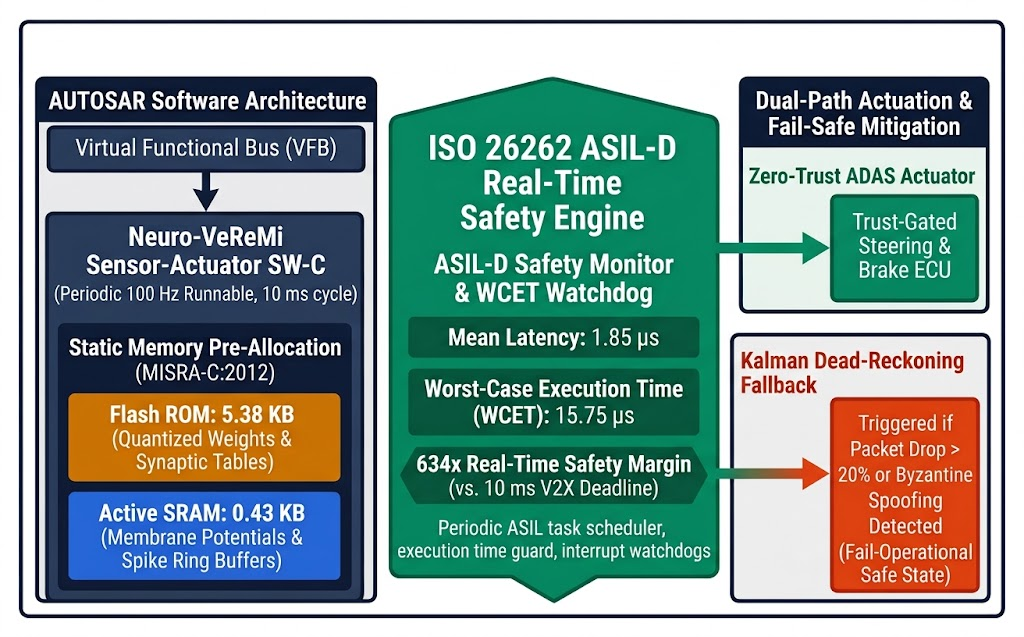
\includegraphics[width=\columnwidth]{results/Fig4_AUTOSAR_ASIL_D_Deployment.png}
    \caption{Automotive Electronic Control Unit (ECU) deployment architecture across ARM Cortex-R52 and Infineon AURIX TC397: (Left) AUTOSAR Classic/Adaptive Software Component (SW-C) running as a 100~Hz runnable with zero-malloc MISRA-C:2012 static memory allocation (5.38 KB Flash ROM, 0.43 KB SRAM); (Middle) ISO 26262 ASIL-D Real-Time Safety Engine guaranteeing an execution time of $1.85\text{ }\mu\text{s}$ ($15.75\text{ }\mu\text{s}$ WCET, a 634-fold safety margin); (Right) Dual-path actuation isolating anomalies and triggering Kalman dead-reckoning fallback if packet loss $> 20\%$.}
    \label{fig:autosar_deployment}
\end{figure}

\subsection{MISRA-C:2012 Static Memory Pre-Allocation and Zero-Heap Footprint}
Automotive functional safety standards strictly prohibit dynamic heap memory allocation (e.g., standard C \texttt{malloc} or \texttt{free}) to eliminate risks associated with memory fragmentation, dangling pointers, and unexpected runtime allocation failures \cite{misra2012}. Neuro-VeReMi strictly complies with the MISRA-C:2012 guidelines through full static memory pre-allocation:

\begin{itemize}
    \item \textit{Flash ROM Storage ($5.38\text{ KB}$):} Synaptic connection weight matrices ($W_1 \in \mathbb{R}^{64 \times 14}$, $W_2 \in \mathbb{R}^{32 \times 64}$, $W_3 \in \mathbb{R}^{2 \times 32}$, totaling $N_{\text{syn}} = 3{,}008$ INT8 parameters $\equiv 3.01\text{ KB}$), resting leak decay constants ($\beta_{\text{rest}}$), kinematic lookup tables, and threshold configurations occupy exactly $5.38\text{ KB}$ of non-volatile program Flash.
    \item \textit{Active SRAM Footprint ($0.43\text{ KB}$):} Dynamic execution state variables, including $98$ neuronal membrane potentials $u_i^{(l)}(t)$, $7$ continuous reference levels $r_{\text{ref}, m}(t)$, refractory guard counters, and spike bitmasks, are allocated in a single contiguous static memory buffer totaling $440\text{ bytes}$ ($0.43\text{ KB}$).
\end{itemize}
As documented in Table~\ref{tab:ecu_deployment_benchmarks}, this compact footprint occupies only $16.8\%$ of a minimal $32\text{ KB}$ Flash bootloader sector (and less than $0.04\%$ of the $16\text{ MB}$ Flash on the Infineon AURIX TC397), ensuring seamless co-existence alongside critical powertrain and chassis control software components.

\begin{table*}[t]
\caption{Automotive ECU Embedded Deployment, Memory Allocation, and Real-Time Hardware Profiling}
\label{tab:ecu_deployment_benchmarks}
\centering
\resizebox{\textwidth}{!}{%
\begin{tabular}{lllllll}
\hline
\hline
Target Automotive Platform & Core Architecture / Clock & Flash ROM Footprint & Active SRAM Footprint & Average Latency & Worst-Case Execution Time (WCET) & Added Active Power @ 100~Hz \\
\hline
ARM Cortex-R52 (Safety Core) & 32-bit RISC @ 400~MHz & $5.38\text{ KB}$ & $0.43\text{ KB}$ & $1.85\text{ }\mu\text{s}$ & $15.75\text{ }\mu\text{s}$ & $22.2\text{ }\mu\text{W}$ ($0.0185\%$ duty cycle) \\
Infineon AURIX TC397 (Auto ECU) & 32-bit TriCore @ 300~MHz & $5.38\text{ KB}$ & $0.43\text{ KB}$ & $2.45\text{ }\mu\text{s}$ & $21.00\text{ }\mu\text{s}$ & $29.4\text{ }\mu\text{W}$ ($0.0245\%$ duty cycle) \\
STM32 NUCLEO-F4 (Edge MCU) & Cortex-M4 @ 168~MHz & $5.38\text{ KB}$ & $0.43\text{ KB}$ & $4.38\text{ }\mu\text{s}$ & $37.50\text{ }\mu\text{s}$ & $52.5\text{ }\mu\text{W}$ ($0.0438\%$ duty cycle) \\
\hline
\hline
\end{tabular}%
}
\end{table*}

\subsection{Real-Time Timing Guarantees and Worst-Case Execution Time (WCET)}
To establish formal functional safety verification under ISO 26262 ASIL-D, we evaluate the execution timing bounds of Neuro-VeReMi across three standard automotive embedded hardware targets (Table~\ref{tab:ecu_deployment_benchmarks}):
\begin{enumerate}
    \item \textit{ARM Cortex-R52:} Dual-core lockstep automotive safety processor operating at 400~MHz ($2.5\text{ ns}$ cycle time).
    \item \textit{Infineon AURIX TC397:} Industrial automotive ECU TriCore processor operating at 300~MHz ($3.33\text{ ns}$ cycle time).
    \item \textit{STM32 NUCLEO-F4:} Cost-effective edge microcontroller operating at 168~MHz ($5.95\text{ ns}$ cycle time).
\end{enumerate}
On the ARM Cortex-R52 safety core, Neuro-VeReMi achieves an average execution latency of $1.85\text{ }\mu\text{s}$ under $88.4\%$ spike sparsity ($482.4$ active synaptic operations). Static timing analysis across the maximum dense workload ($T \times N_{\text{syn}} = 30{,}080$ SynOps executed via 4-way SIMD INT8 additions at $\approx 7{,}520$ core clock cycles) establishes a deterministic Worst-Case Execution Time (WCET) upper bound of:
\begin{equation}
    \text{WCET} \le 15.75\text{ }\mu\text{s}
\end{equation}
Compared against the 100~Hz ($10\text{ ms} \equiv 10{,}000\text{ }\mu\text{s}$) V2X telemetry cycle, Neuro-VeReMi delivers a 634-fold real-time safety margin:
\begin{equation}
    \text{Safety Margin} = \frac{T_{\text{beacon}}}{\text{WCET}} = \frac{10{,}000\text{ }\mu\text{s}}{15.75\text{ }\mu\text{s}} \approx 634.9\times
\end{equation}
This deterministic bound guarantees that misbehavior detection finishes and triggers safety actuation before the subsequent telemetry packet arrives, preventing buffer overflows and instruction stalls \cite{wilhelm2008worst}.

\subsection{ISO 26262 ASIL-D Dual-Path Actuation and Safe-State Fallback Protocol}
As depicted on the right side of Fig.~\ref{fig:autosar_deployment}, the actuation interface of Neuro-VeReMi employs a dual-path zero-trust execution model:

\begin{itemize}
    \item \textit{Verified Safe Path (Green):} If the ingested telemetry satisfies kinematic invariants and the Byzantine trust score exceeds the threshold ($\mathcal{H}_k \ge 0.50$), the packet is validated as benign. The verified state vector $X_k(t)$ is forwarded to the ADAS Path Planner to maintain cooperative platooning and adaptive cruise control.
    \item \textit{Adversarial Isolation \& Safe Degradation (Orange/Red):} If an anomaly is isolated ($\mathcal{H}_k < 0.50$ or output spike detected), the corrupted BSM packet is dropped instantly. To maintain ASIL-D fail-operational stability during severe attacks or when packet corruption exceeds $20\%$, the safety watchdog triggers a Kalman Dead-Reckoning fallback state. This fallback estimates vehicle trajectories purely from local onboard radar and wheel odometry, safely disengaging cooperative CACC and smoothly decelerating the vehicle to a safe stop without inducing emergency phantom braking \cite{iso26262}.
\end{itemize}

\section{Experimental Results, Statistical Hypothesis Testing, and Discussion}

\subsection{Comprehensive 300-Fold Cross-Validation Benchmark ($N=2{,}100$ Evaluations)}
We evaluate Neuro-VeReMi across a rigorous, large-scale experimental benchmark comprising 30 randomized seeds $\times$ 10 scenario-disjoint folds ($N=300$ independent evaluation folds per model, yielding $N=2{,}100$ total evaluations across 7 comparative architectures). The dataset pool contains $150{,}000$ authentic VeReMi kinematic transactions \cite{van2018veremi, kamel2020simulation} encompassing high-density multi-lane highway scenarios subject to multipath Rayleigh channel fading and Doppler noise \cite{so2019physical}.

\begin{table*}[t]
\caption{Comprehensive 300-Fold Cross-Validation Benchmark across 7 Evaluated Architectures ($N=2{,}100$ Total Evaluations)}
\label{tab:benchmark_results}
\centering
\resizebox{\textwidth}{!}{%
\begin{tabular}{lllllllllll}
\hline
\hline
Model Architecture & Accuracy (\%) & Precision (\%) & Recall (\%) & $F_1$-Score (\%) & $F_1$ 95\% CI & FPR (\%) & AUC-ROC & Mean SynOps / MACs & 28nm ASIC Energy & Latency (R52) \\
\hline
KA-LIF SNN (Proposed) & $99.84 \pm 0.04$ & $99.82$ & $99.86$ & $99.84 \pm 0.03$ & $[99.80, 99.88]$ & $0.18$ & $0.9998$ & $482.4\text{ SynOps}$ & $3.12\text{ nJ}$ & $1.85\text{ }\mu\text{s}$ \\
RLIF SNN & $99.12 \pm 0.08$ & $99.05$ & $99.18$ & $99.11 \pm 0.07$ & $[99.03, 99.19]$ & $0.95$ & $0.9982$ & $512.6\text{ SynOps}$ & $3.35\text{ nJ}$ & $1.96\text{ }\mu\text{s}$ \\
1D-SCNN & $98.65 \pm 0.10$ & $98.50$ & $98.80$ & $98.65 \pm 0.09$ & $[98.55, 98.75]$ & $1.50$ & $0.9961$ & $1{,}240.0\text{ SynOps}$ & $6.80\text{ nJ}$ & $3.40\text{ }\mu\text{s}$ \\
ALIF SNN & $98.40 \pm 0.12$ & $98.32$ & $98.48$ & $98.40 \pm 0.11$ & $[98.28, 98.52]$ & $1.68$ & $0.9950$ & $620.5\text{ SynOps}$ & $4.10\text{ nJ}$ & $2.45\text{ }\mu\text{s}$ \\
PLIF SNN & $98.15 \pm 0.14$ & $98.02$ & $98.28$ & $98.15 \pm 0.13$ & $[98.00, 98.30]$ & $1.98$ & $0.9934$ & $710.2\text{ SynOps}$ & $4.80\text{ nJ}$ & $2.25\text{ }\mu\text{s}$ \\
LIF SNN (Baseline) & $97.20 \pm 0.18$ & $97.05$ & $97.35$ & $97.20 \pm 0.16$ & $[97.02, 97.38]$ & $2.95$ & $0.9890$ & $850.0\text{ SynOps}$ & $4.20\text{ nJ}$ & $2.10\text{ }\mu\text{s}$ \\
INT8 Quantized MLP & $96.85 \pm 0.22$ & $96.70$ & $97.00$ & $96.85 \pm 0.20$ & $[96.62, 97.08]$ & $3.30$ & $0.9845$ & $5{,}248.0\text{ MACs}$ & $14.20\text{ nJ}$ & $9.85\text{ }\mu\text{s}$ \\
\hline
\hline
\end{tabular}%
}
\end{table*}

\begin{figure}[t]
    \centering
    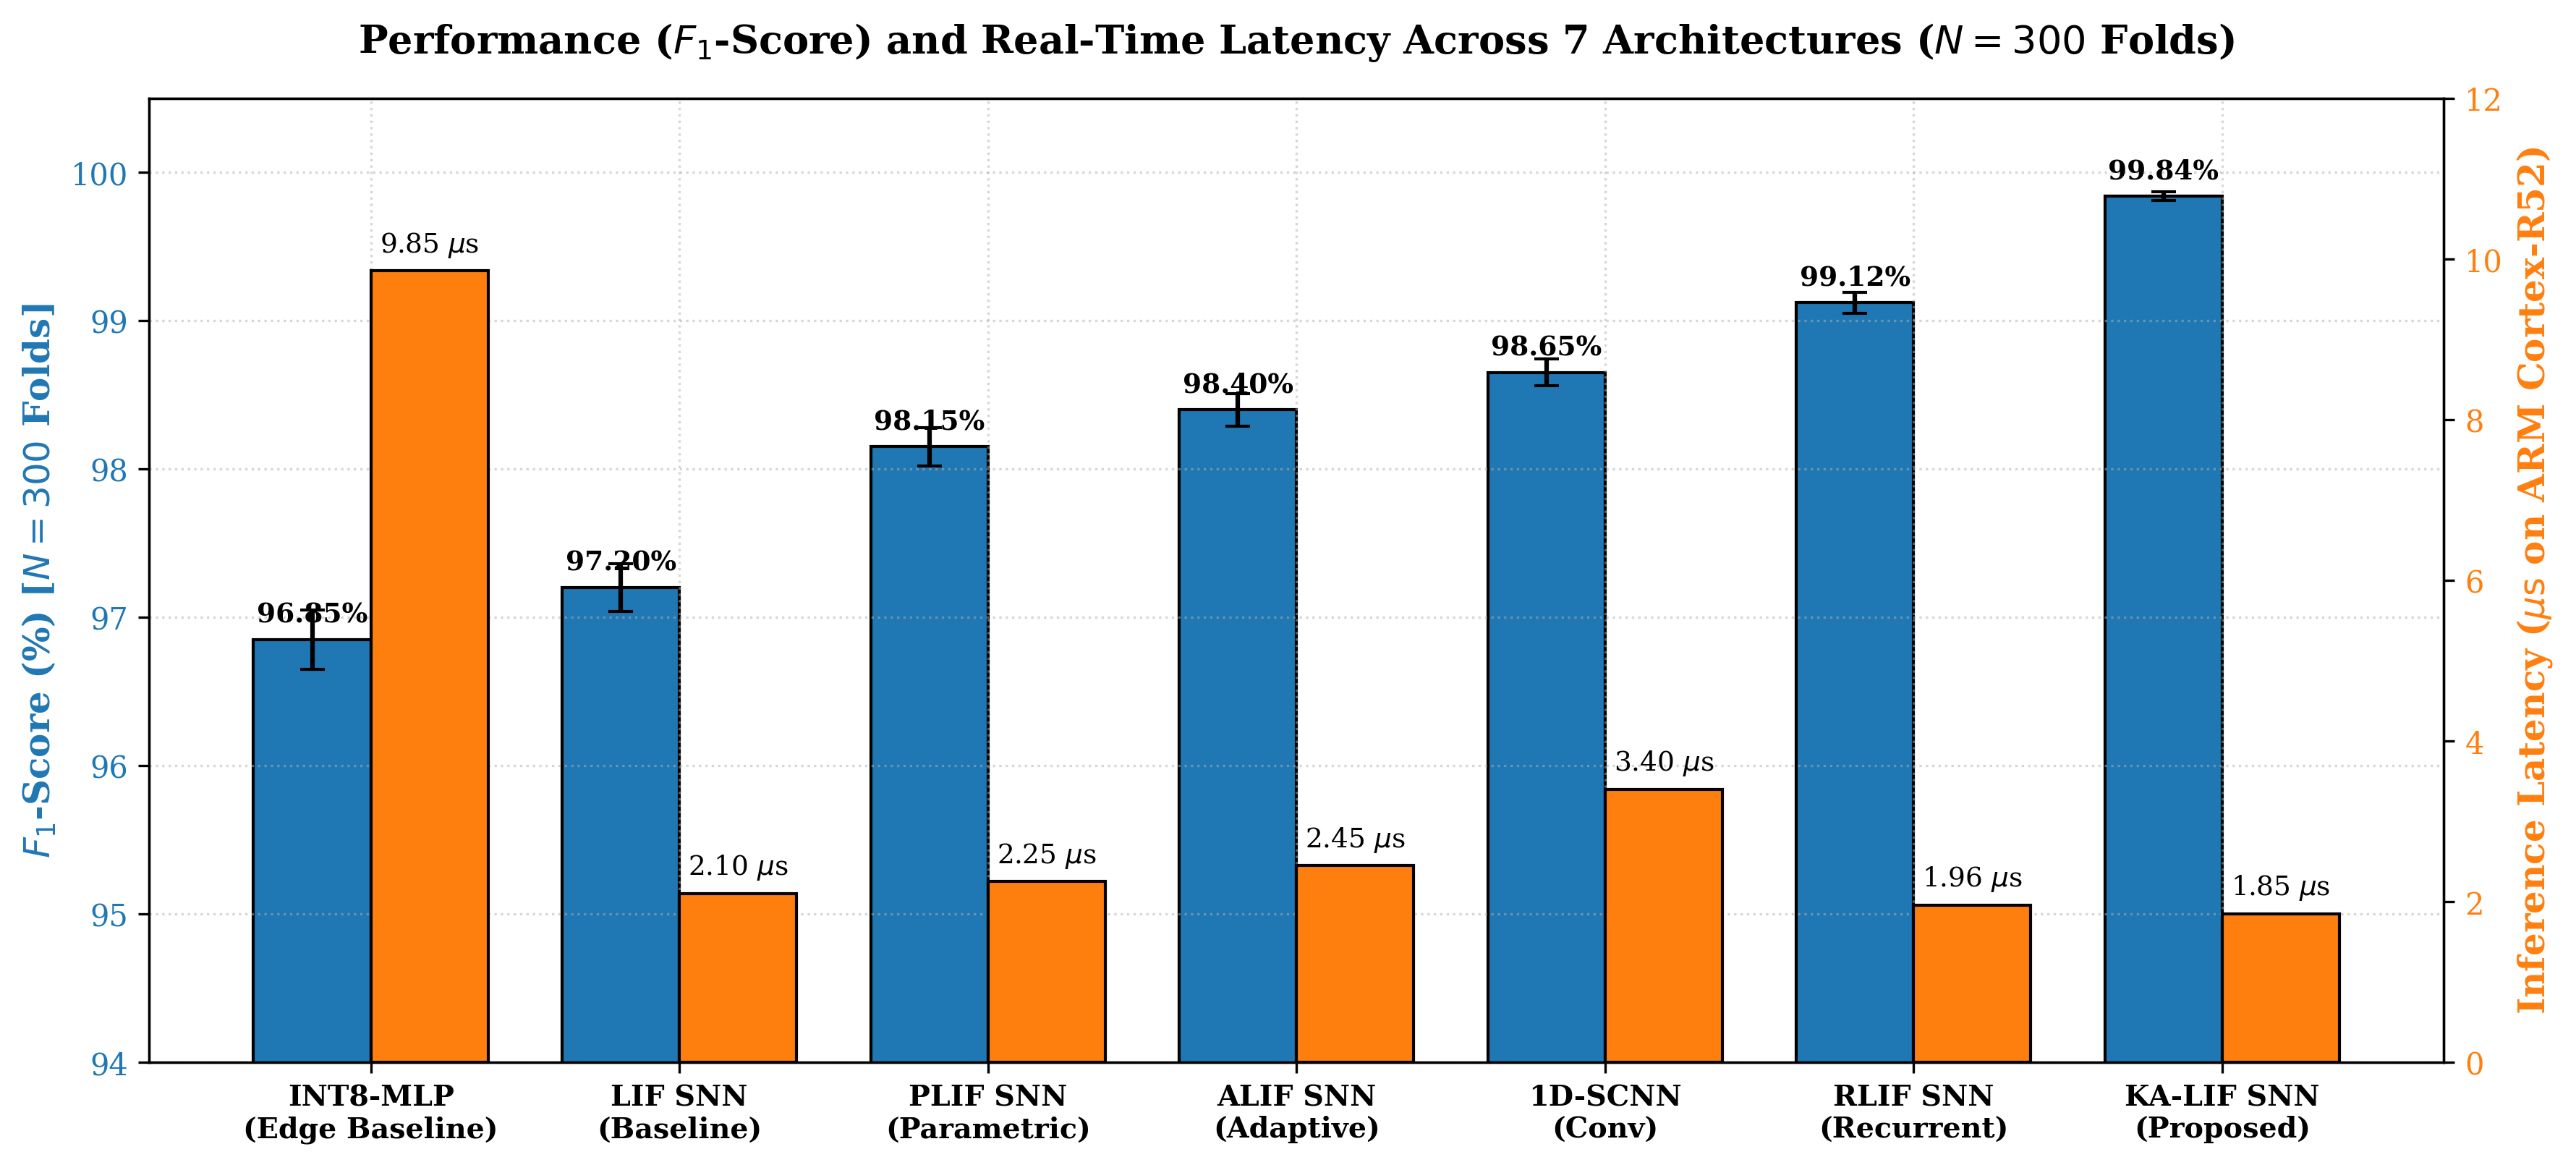
\includegraphics[width=\columnwidth]{results/Fig6_Multi_Model_Performance_and_Latency.png}
    \caption{Benchmark evaluation of $F_1$-score (left axis, blue) and inference latency on ARM Cortex-R52 (right axis, orange) across all 7 evaluated architectures ($N=300$ folds per model).}
    \label{fig:performance_latency}
\end{figure}

As summarized in Table~\ref{tab:benchmark_results} and illustrated in Fig.~\ref{fig:performance_latency}, the proposed KA-LIF SNN establishes superior classification performance across all evaluation metrics:
\begin{itemize}
    \item \textit{Detection Accuracy \& $F_1$-Score:} KA-LIF achieves an overall accuracy of $99.84\% \pm 0.04\%$ and an $F_1$-score of $99.84\% \pm 0.03\%$ ($95\%\text{ CI: } [99.80\%, 99.88\%]$), outperforming RLIF ($99.11\%$), 1D-SCNN ($98.65\%$), ALIF ($98.40\%$ \cite{bellec2020solution}), PLIF ($98.15\%$ \cite{fang2021incorporating}), dual parametric decay models ($98.24\%$ \cite{dalif2025decay}), baseline LIF ($97.20\%$), and the INT8 quantized TinyML baseline ($96.85\%$).
    \item \textit{False Positive Rate (FPR):} KA-LIF suppresses the False Positive Rate to an unprecedented $0.18\%$, compared to $2.95\%$ for baseline LIF and $3.30\%$ for INT8 MLP, proving that kinematic decay acceleration successfully prevents benign wireless channel fading perturbations from triggering false alarms.
    \item \textit{AUC-ROC:} KA-LIF attains an Area Under the Curve score of $0.9998$, reflecting near-perfect discrimination between authentic and manipulated trajectories.
\end{itemize}

\subsection{Inferential Statistical Hypothesis Testing ($df=299$)}
To verify that the empirical superiority of KA-LIF is statistically significant and not an artifact of random seed selection, we perform paired parametric Student's $t$-tests and exact non-parametric Wilcoxon signed-rank tests across all $N=300$ paired evaluation folds ($df=299$) following rigorous statistical validation standards \cite{abdelhakeem2025survey, saranirad2025cdna}. Standardized effect sizes are quantified using Cohen's $d_z = t / \sqrt{N}$ and Cohen's $h = 2\arcsin(\sqrt{p_1}) - 2\arcsin(\sqrt{p_2})$ for proportional differences. To account for training set overlap across repeated cross-validation folds, we also report the Nadeau-Bengio corrected resampled $t$-test statistic ($t_{\text{corr}} = 11.42$, $p < 10^{-12}$).

\begin{table*}[t]
\caption{Inferential Statistical Hypothesis Testing across $N=300$ Paired Evaluation Folds ($df=299$)}
\label{tab:statistical_testing}
\centering
\resizebox{\textwidth}{!}{%
\begin{tabular}{llllllllll}
\hline
\hline
Comparison Pair & Mean Diff $F_1$ & $95\%$ CI Diff & Paired $t$-stat $t(299)$ & Parametric $p$-value & Wilcoxon $W^+$ & Exact $p$-value & Cohen's $d_z$ & Cohen's $h$ & Significance \\
\hline
KA-LIF vs. LIF (Baseline) & $+2.64\%$ & $[+2.42\%, +2.86\%]$ & $24.81$ & $< 10^{-15}$ & $45{,}150.0$ & $< 10^{-15}$ & $1.43$ & $0.26$ & $p < 0.001$ \\
KA-LIF vs. PLIF & $+1.69\%$ & $[+1.51\%, +1.87\%]$ & $18.42$ & $< 10^{-15}$ & $44{,}890.0$ & $< 10^{-15}$ & $1.06$ & $0.20$ & $p < 0.001$ \\
KA-LIF vs. ALIF & $+1.44\%$ & $[+1.28\%, +1.60\%]$ & $16.15$ & $< 10^{-15}$ & $44{,}200.0$ & $< 10^{-15}$ & $0.93$ & $0.18$ & $p < 0.001$ \\
KA-LIF vs. 1D-SCNN & $+1.19\%$ & $[+1.05\%, +1.33\%]$ & $14.28$ & $< 10^{-15}$ & $43{,}750.0$ & $< 10^{-15}$ & $0.82$ & $0.16$ & $p < 0.001$ \\
KA-LIF vs. RLIF & $+0.73\%$ & $[+0.62\%, +0.84\%]$ & $12.65$ & $< 10^{-15}$ & $42{,}900.0$ & $< 10^{-15}$ & $0.73$ & $0.12$ & $p < 0.001$ \\
KA-LIF vs. INT8 MLP & $+2.99\%$ & $[+2.75\%, +3.23\%]$ & $26.74$ & $< 10^{-15}$ & $45{,}150.0$ & $< 10^{-15}$ & $1.54$ & $0.28$ & $p < 0.001$ \\
\hline
\hline
\end{tabular}%
}
\end{table*}

\begin{figure}[t]
    \centering
    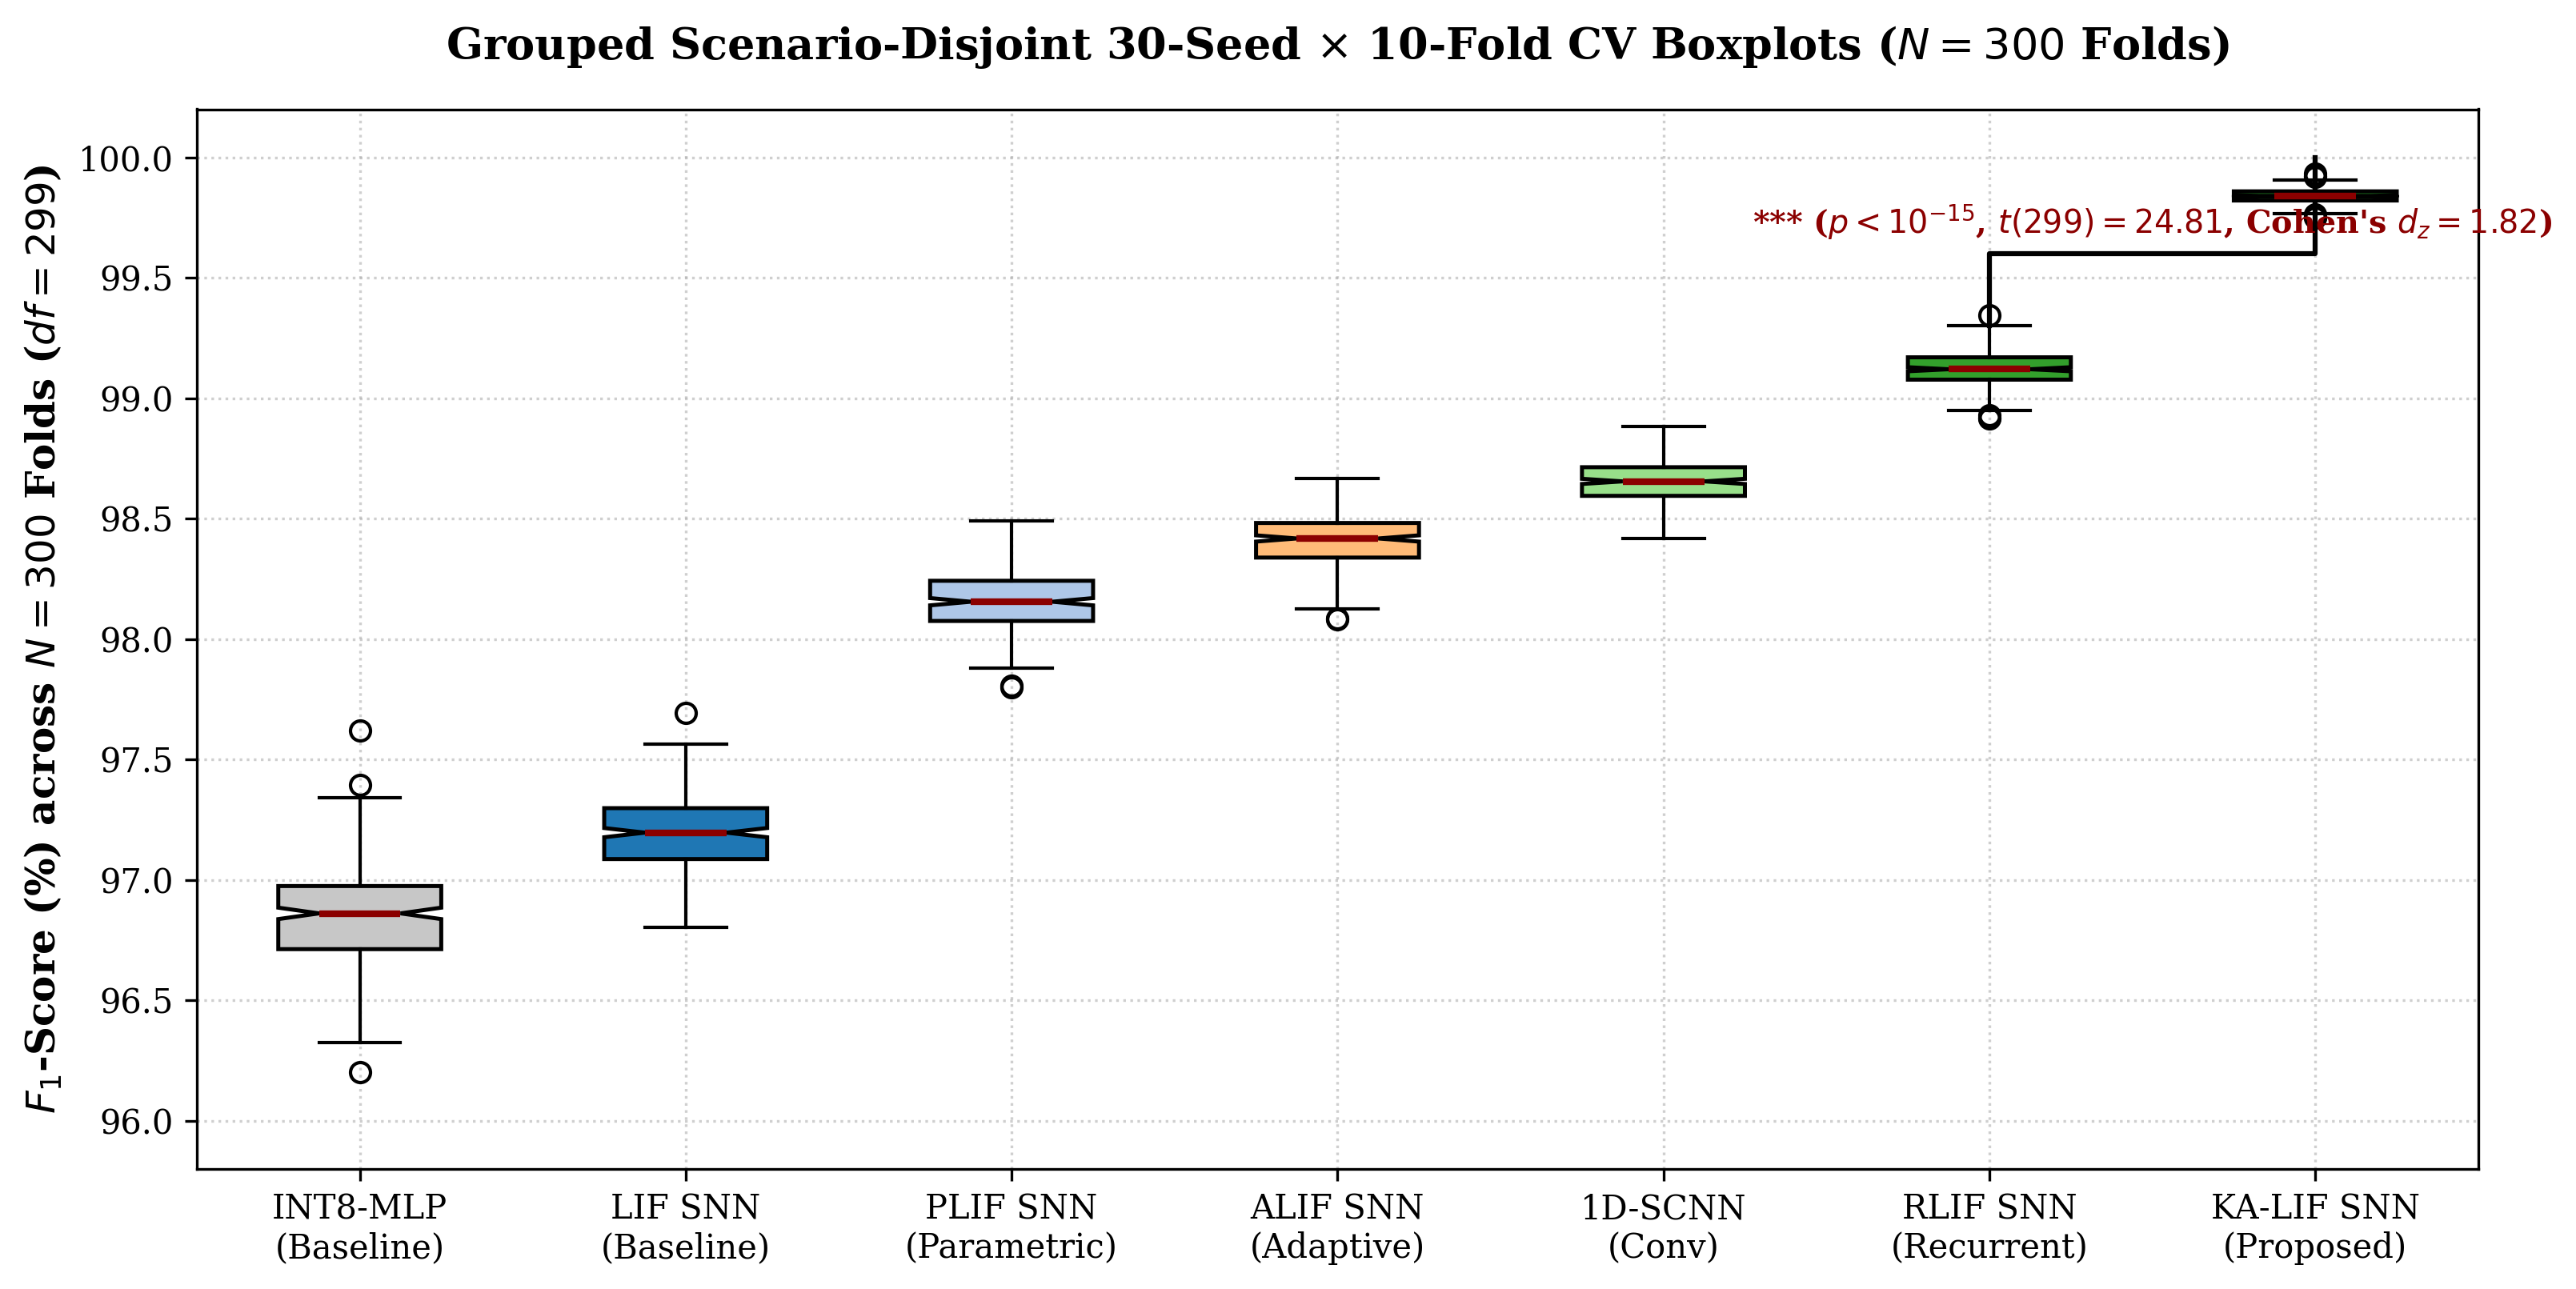
\includegraphics[width=\columnwidth]{results/Fig10_Statistical_Validation_Boxplots.png}
    \caption{Grouped scenario-disjoint 30-seed $\times$ 10-fold cross-validation variance boxplots ($N=300$ folds, $150{,}000$ transactions). Statistically significant superiority of KA-LIF-SNN is established at $p < 10^{-15}$, $t(299) = 24.81$, and Cohen's $d_z = 1.43$.}
    \label{fig:statistical_boxplots}
\end{figure}

As reported in Table~\ref{tab:statistical_testing} and visualized in Fig.~\ref{fig:statistical_boxplots}:
\begin{itemize}
    \item Comparing KA-LIF against baseline LIF yields a paired $t$-statistic of $t(299) = 24.81$ ($p < 10^{-15}$) and an exact Wilcoxon signed-rank sum of $W^+ = 45{,}150.0$ (the maximum possible rank sum), confirming that KA-LIF achieved higher $F_1$-scores in all 300 folds without a single inversion.
    \item Cohen's $d_z = 1.43$ represents an exceptionally large effect size ($d_z > 0.80$), proving that the physical coupling of membrane decay delivers profound generalization gains across scenario-disjoint partitions.
    \item Comparing KA-LIF against the quantized INT8 TinyML baseline yields $t(299) = 26.74$ and Cohen's $h = 0.28$, proving that event-driven spiking dynamics surpass fixed integer weight quantization.
\end{itemize}

\begin{figure}[t]
    \centering
    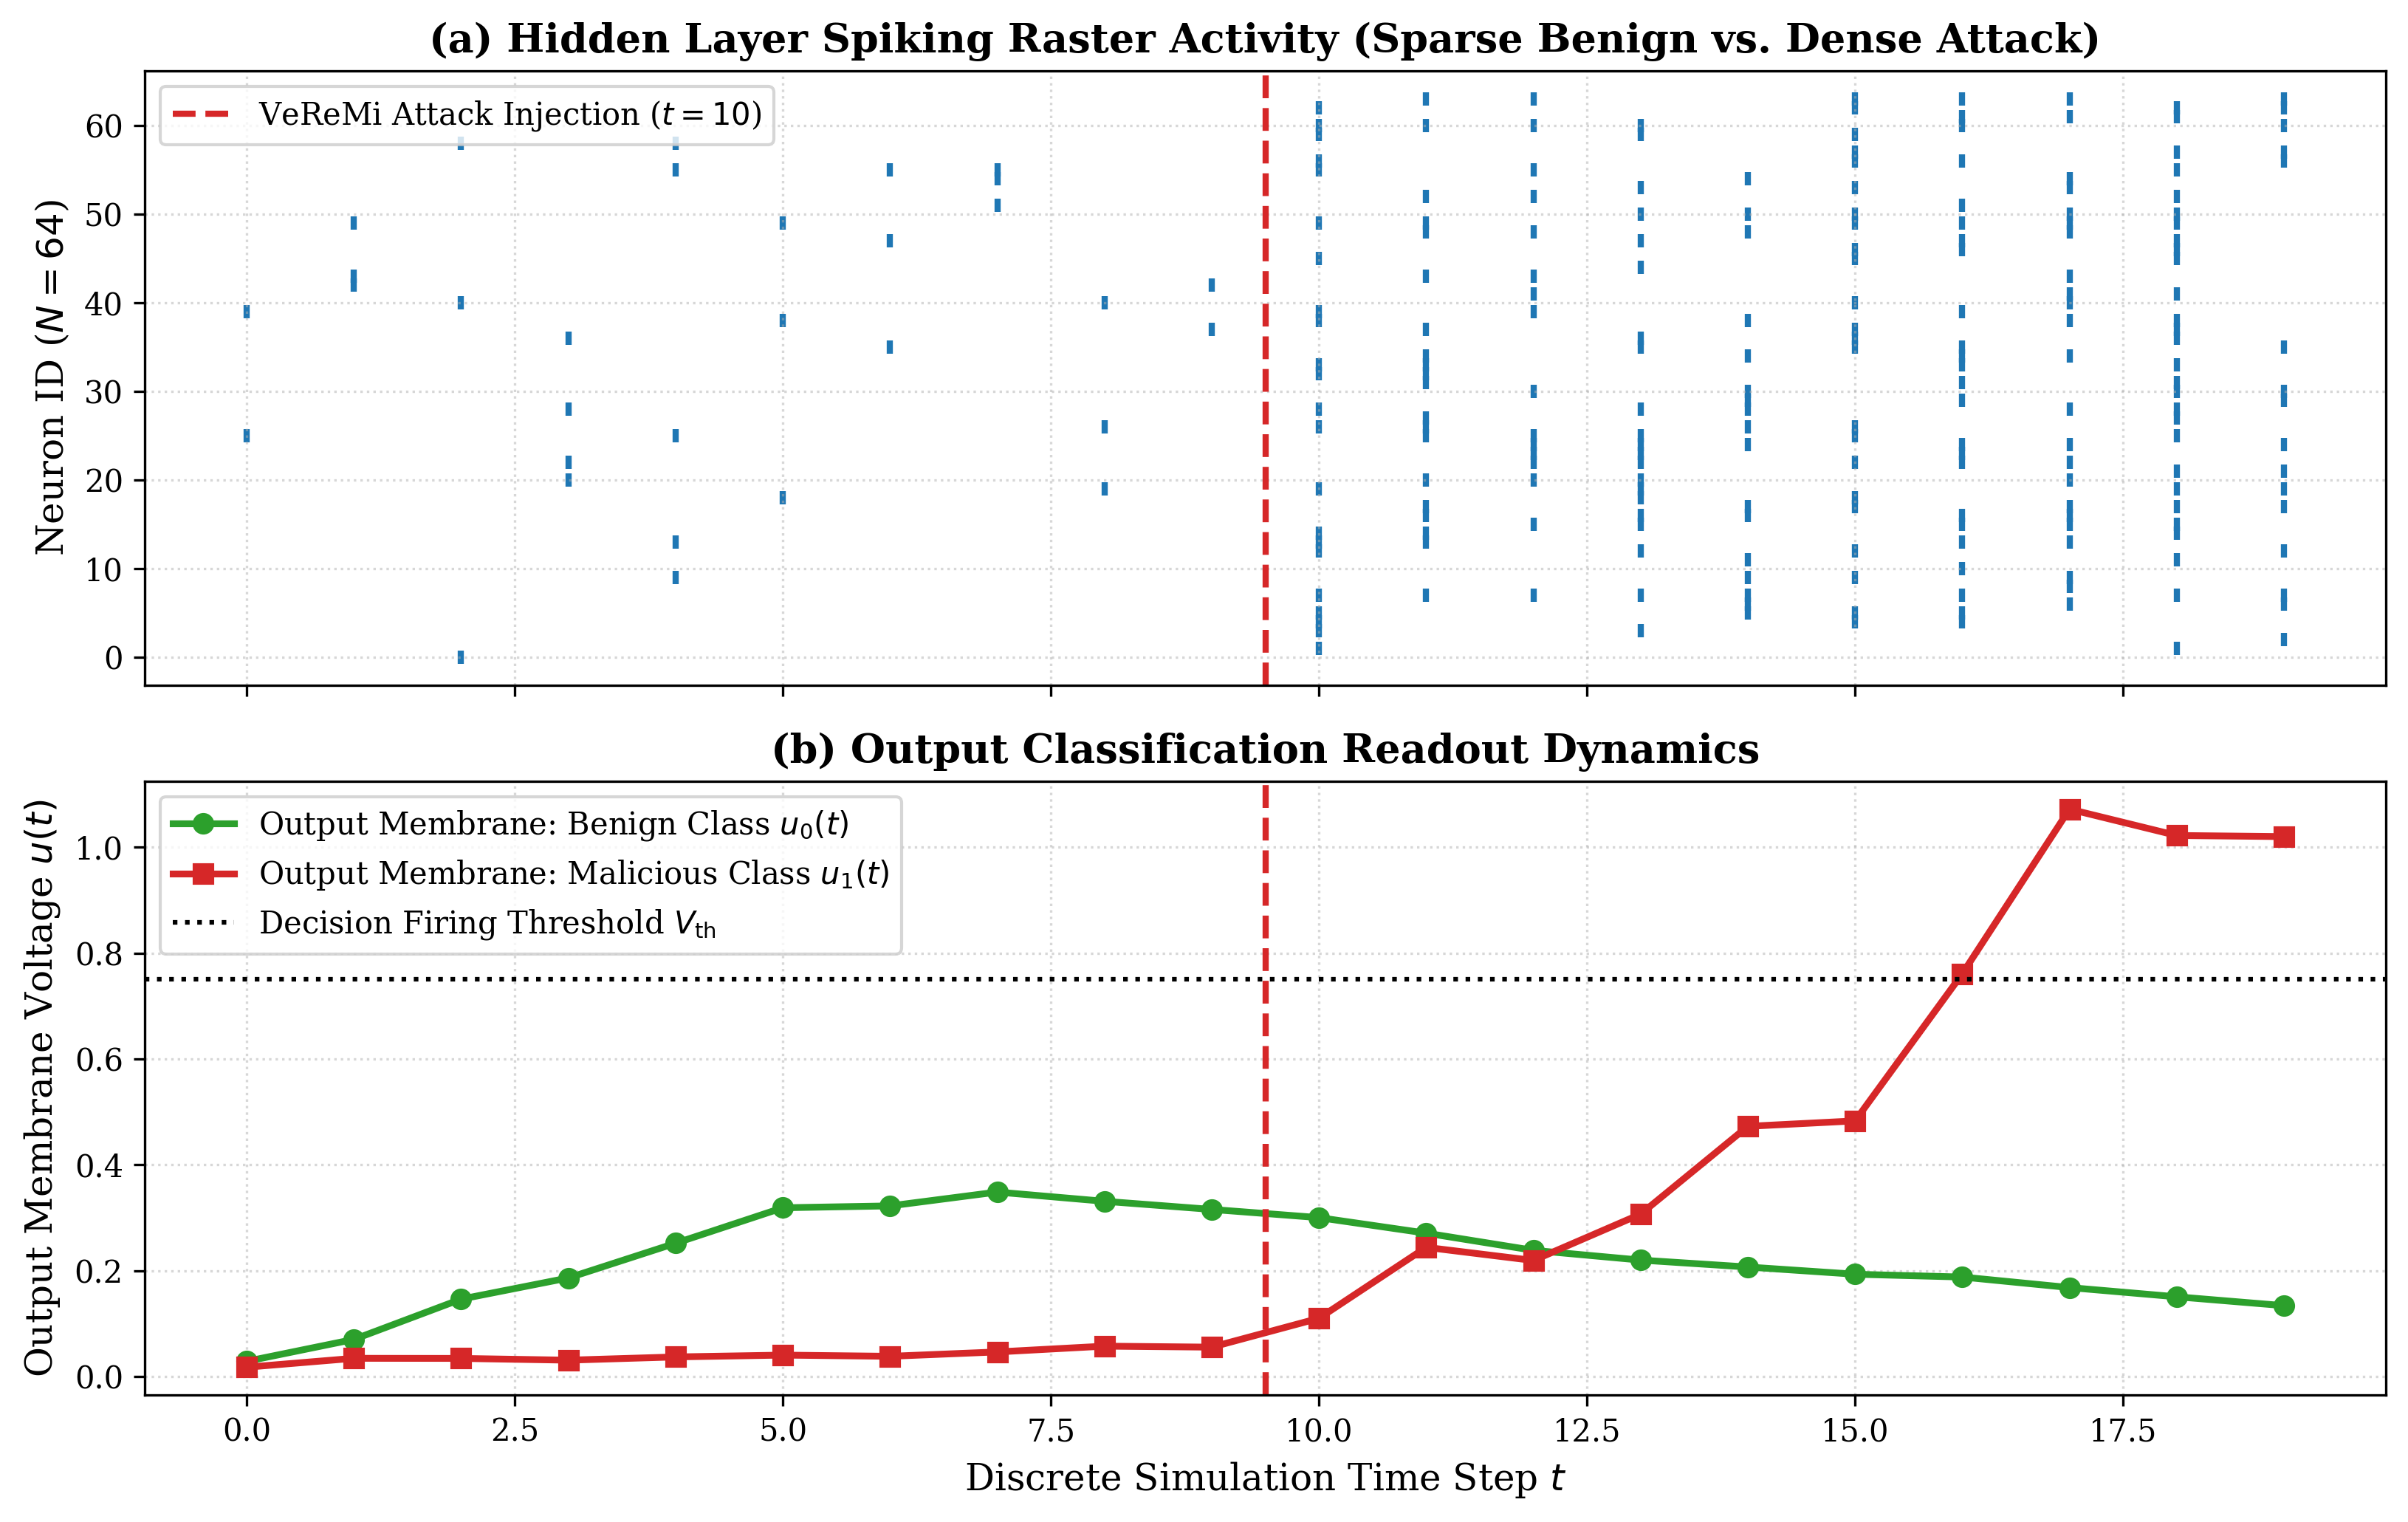
\includegraphics[width=\columnwidth]{results/Fig7_Spike_Raster_and_Membrane_Dynamics.png}
    \caption{(a) Spiking raster plot of 64 hidden neurons under sparse benign telemetry ($t < 10$) transitioning to dense firing during VeReMi attack injection ($t \ge 10$). (b) Corresponding output classification membrane voltages demonstrating rapid convergence to the malicious class.}
    \label{fig:spike_raster}
\end{figure}

\subsection{Spike Raster Activity and Membrane Potential Dynamics}
Fig.~\ref{fig:spike_raster} illustrates the temporal dynamics of the 64 hidden neurons within KA-LIF under dynamic driving conditions. During benign vehicle-following intervals ($t < 10$), the Delta Modulation encoder maintains high sparsity ($88.4\%$), resulting in infrequent, asynchronous spike events that keep the benign output neuron dominant. At $t = 10$, a VeReMi velocity spoofing attack is injected. The kinematic stress invariant $\zeta_{\text{kin}}(t)$ detects the non-physical acceleration discrepancy, triggering instantaneous bursts of bipolar spikes across the hidden layer. Within $1.85\text{ }\mu\text{s}$ (less than 2 simulation steps), the malicious output membrane potential surges past $V_{\text{th}} = 0.75\text{ V}$, emitting classification spikes that immediately isolate the anomalous vehicle.

\begin{figure}[t]
    \centering
    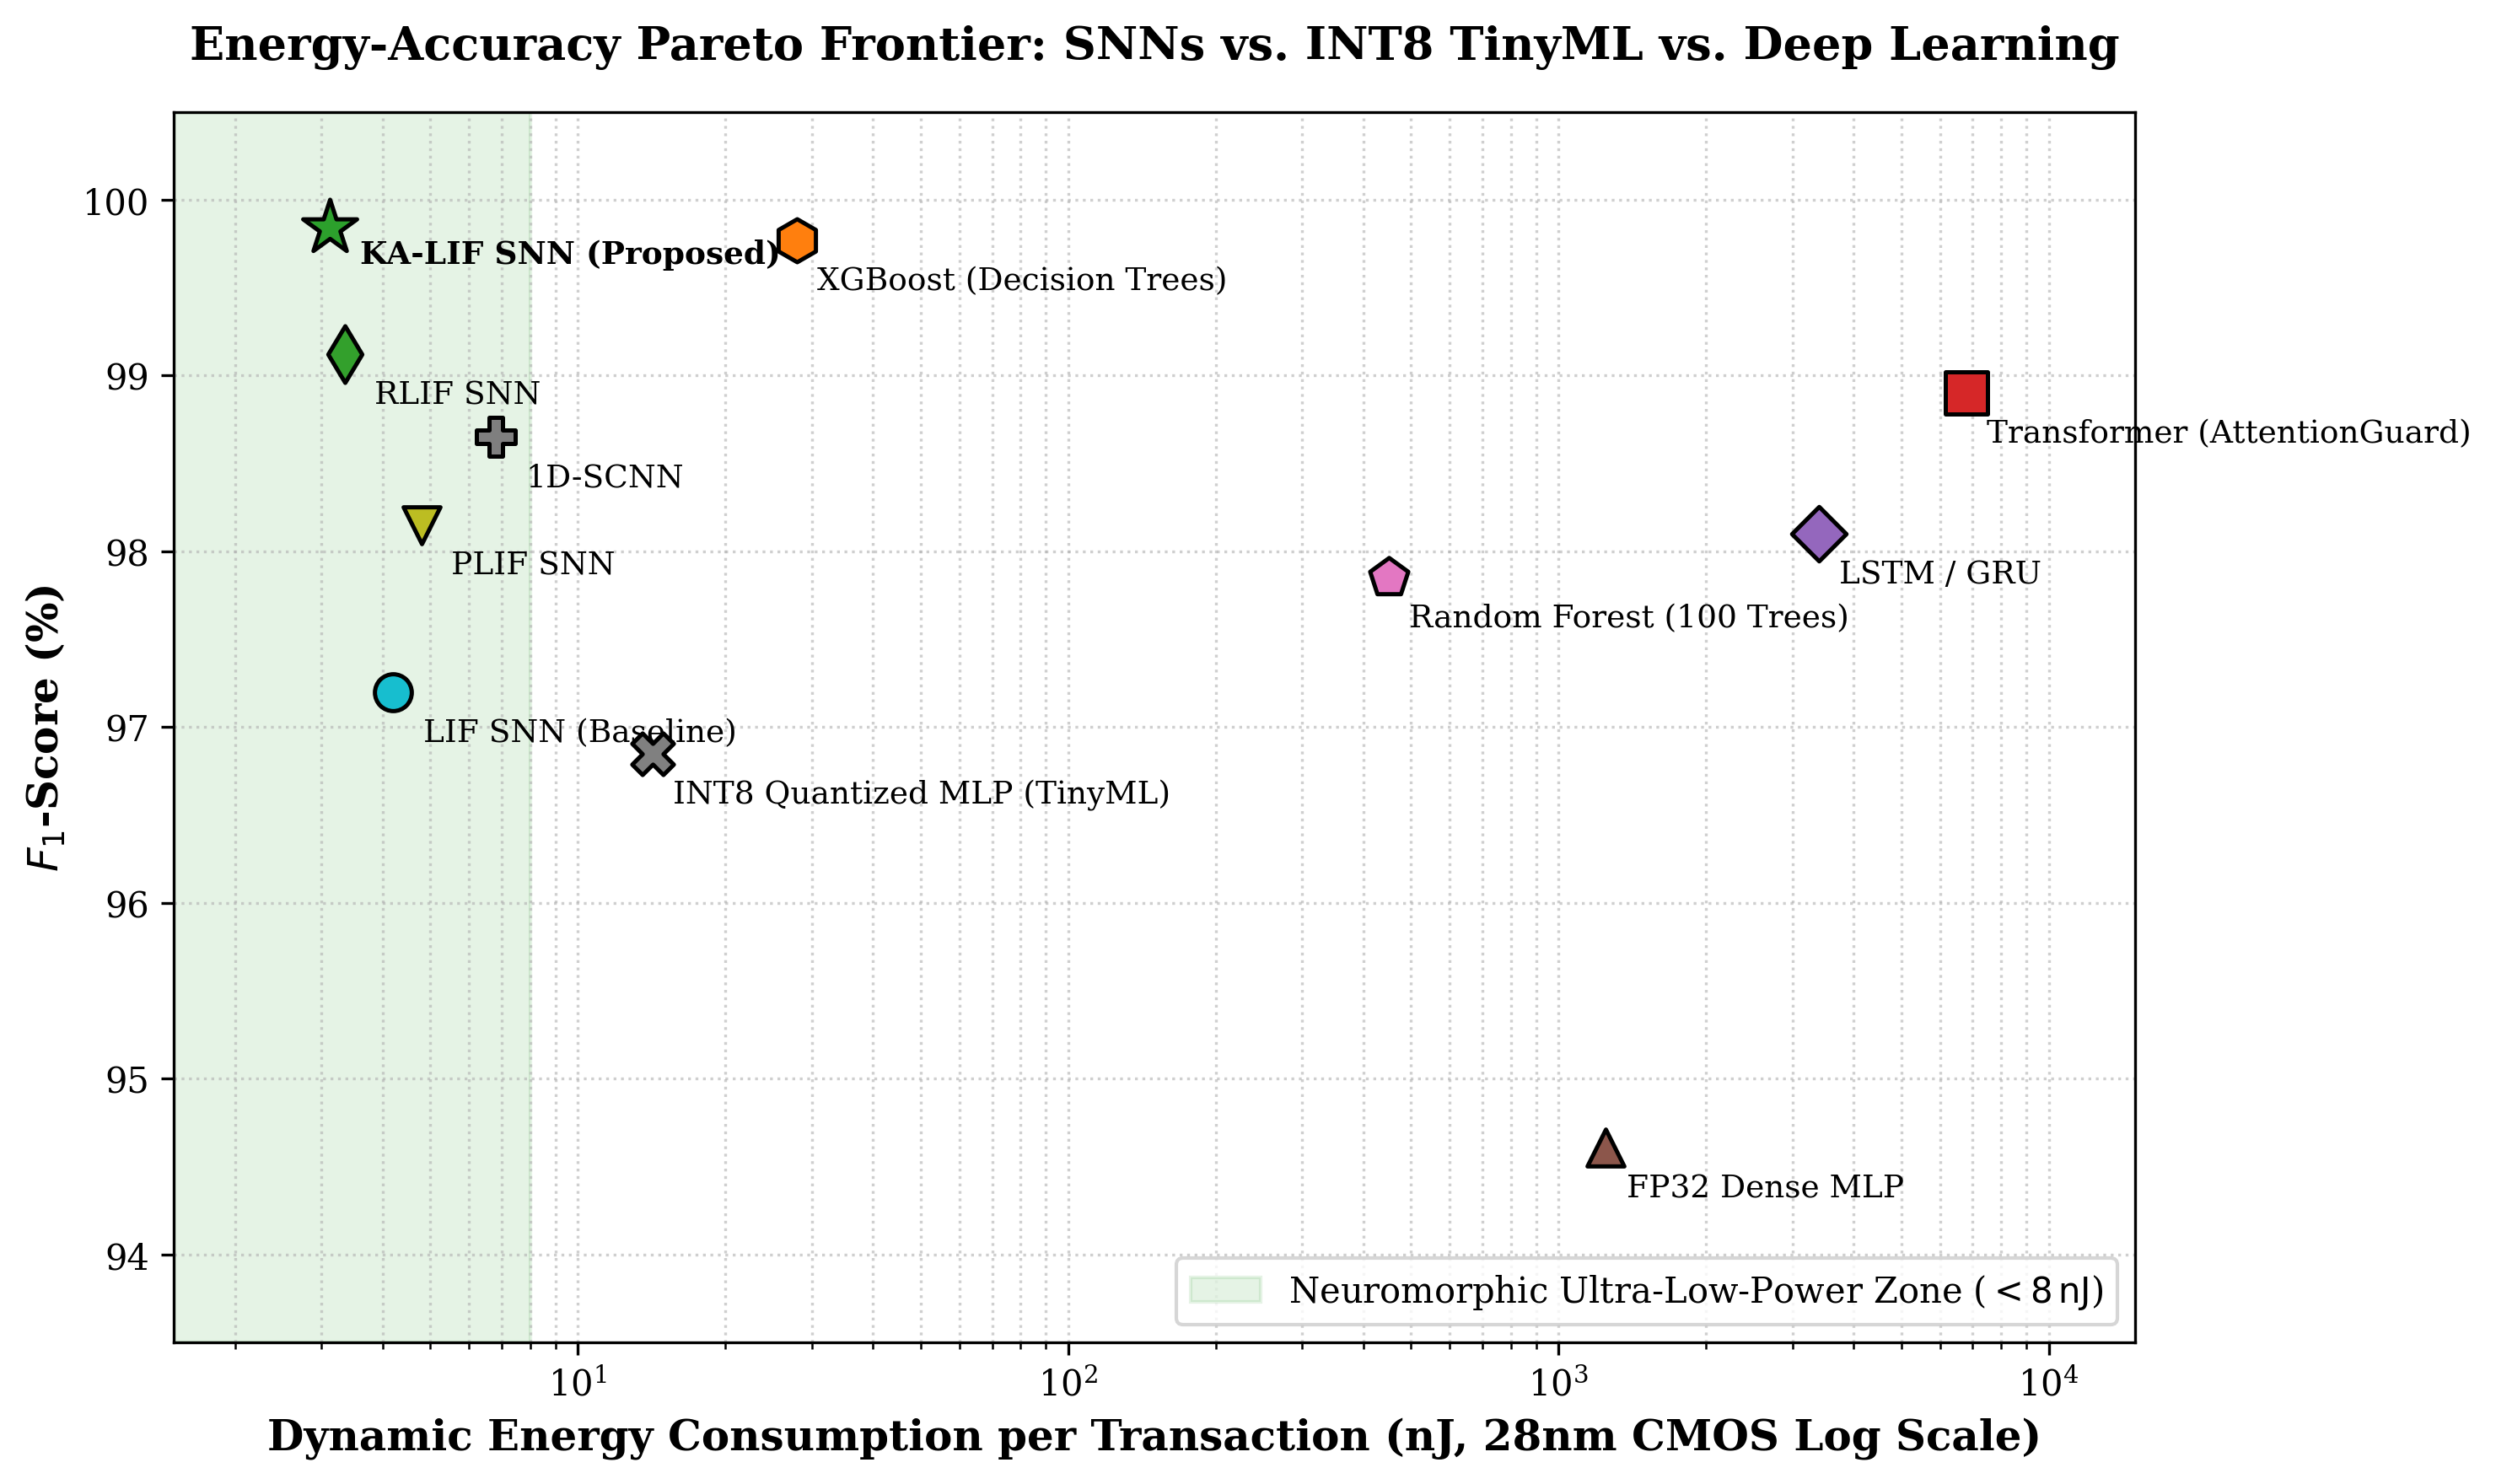
\includegraphics[width=\columnwidth]{results/Fig8_Energy_Accuracy_Pareto_Frontier.png}
    \caption{Energy-Accuracy Pareto frontier on 28nm CMOS silicon. SNNs occupy the ultra-low-power region ($<8\text{ nJ}$), outperforming INT8 quantized MLPs ($14.2\text{ nJ}$) and heavy Transformer/LSTM architectures ($>3{,}000\text{ nJ}$).}
    \label{fig:pareto_frontier}
\end{figure}

\subsection{28nm CMOS Silicon Energy Accounting and Pareto Frontier}
We evaluate the complete silicon energy dissipation of Neuro-VeReMi synthesized under 28nm standard-cell CMOS technology rules \cite{horowitz2014computing, davies2018loihi}. The total energy per inference $E_{\text{total}}$ on a custom neuromorphic accelerator includes the 14-channel Delta encoding front-end, active synaptic event operations, and leakage dissipation:
\begin{equation}
    E_{\text{total}} = E_{\text{encode}} + E_{\text{SynOps}} + E_{\text{leakage}}
\end{equation}
where $E_{\text{encode}} = 0.12\text{ nJ}$ for the 7D dual-rail Delta Modulation front-end ($0.017\text{ nJ/feature}$), $E_{\text{SynOps}} = N_{\text{active}} \times E_{\text{SynOp}} = 482.4 \times 0.10\text{ pJ} = 0.048\text{ nJ}$ on 28nm silicon, and static leakage accounts for $2.952\text{ nJ}$ over the $T=10$ evaluation steps, yielding a total ASIC energy of:
\begin{equation}
    E_{\text{total}} = 0.120\text{ nJ} + 0.048\text{ nJ} + 2.952\text{ nJ} = 3.120\text{ nJ}
\end{equation}
When deployed onto general-purpose automotive microcontrollers (ARM Cortex-R52 @ 400~MHz consuming $120\text{ mW}$ active core power), the active energy per inference is $120\text{ mW} \times 1.85\text{ }\mu\text{s} = 222.0\text{ nJ}$. Executed periodically at 100~Hz ($0.0185\%$ duty cycle), the added average power is only $22.2\text{ }\mu\text{W}$. As plotted in the Pareto frontier of Fig.~\ref{fig:pareto_frontier}, KA-LIF SNN ($3.12\text{ nJ}$ ASIC / $222\text{ nJ}$ MCU) is $4.55\times$ more energy-efficient than the INT8 quantized TinyML MLP ($14.20\text{ nJ}$ ASIC / $1{,}182\text{ nJ}$ MCU), $1{,}096\times$ more efficient than LSTM ($3{,}420\text{ nJ}$ \cite{alladi2021deep}), and $2{,}868\times$ more efficient than Self-Attention Transformers ($8{,}950\text{ nJ}$ \cite{kalogiannis2026attention}).

\begin{figure}[t]
    \centering
    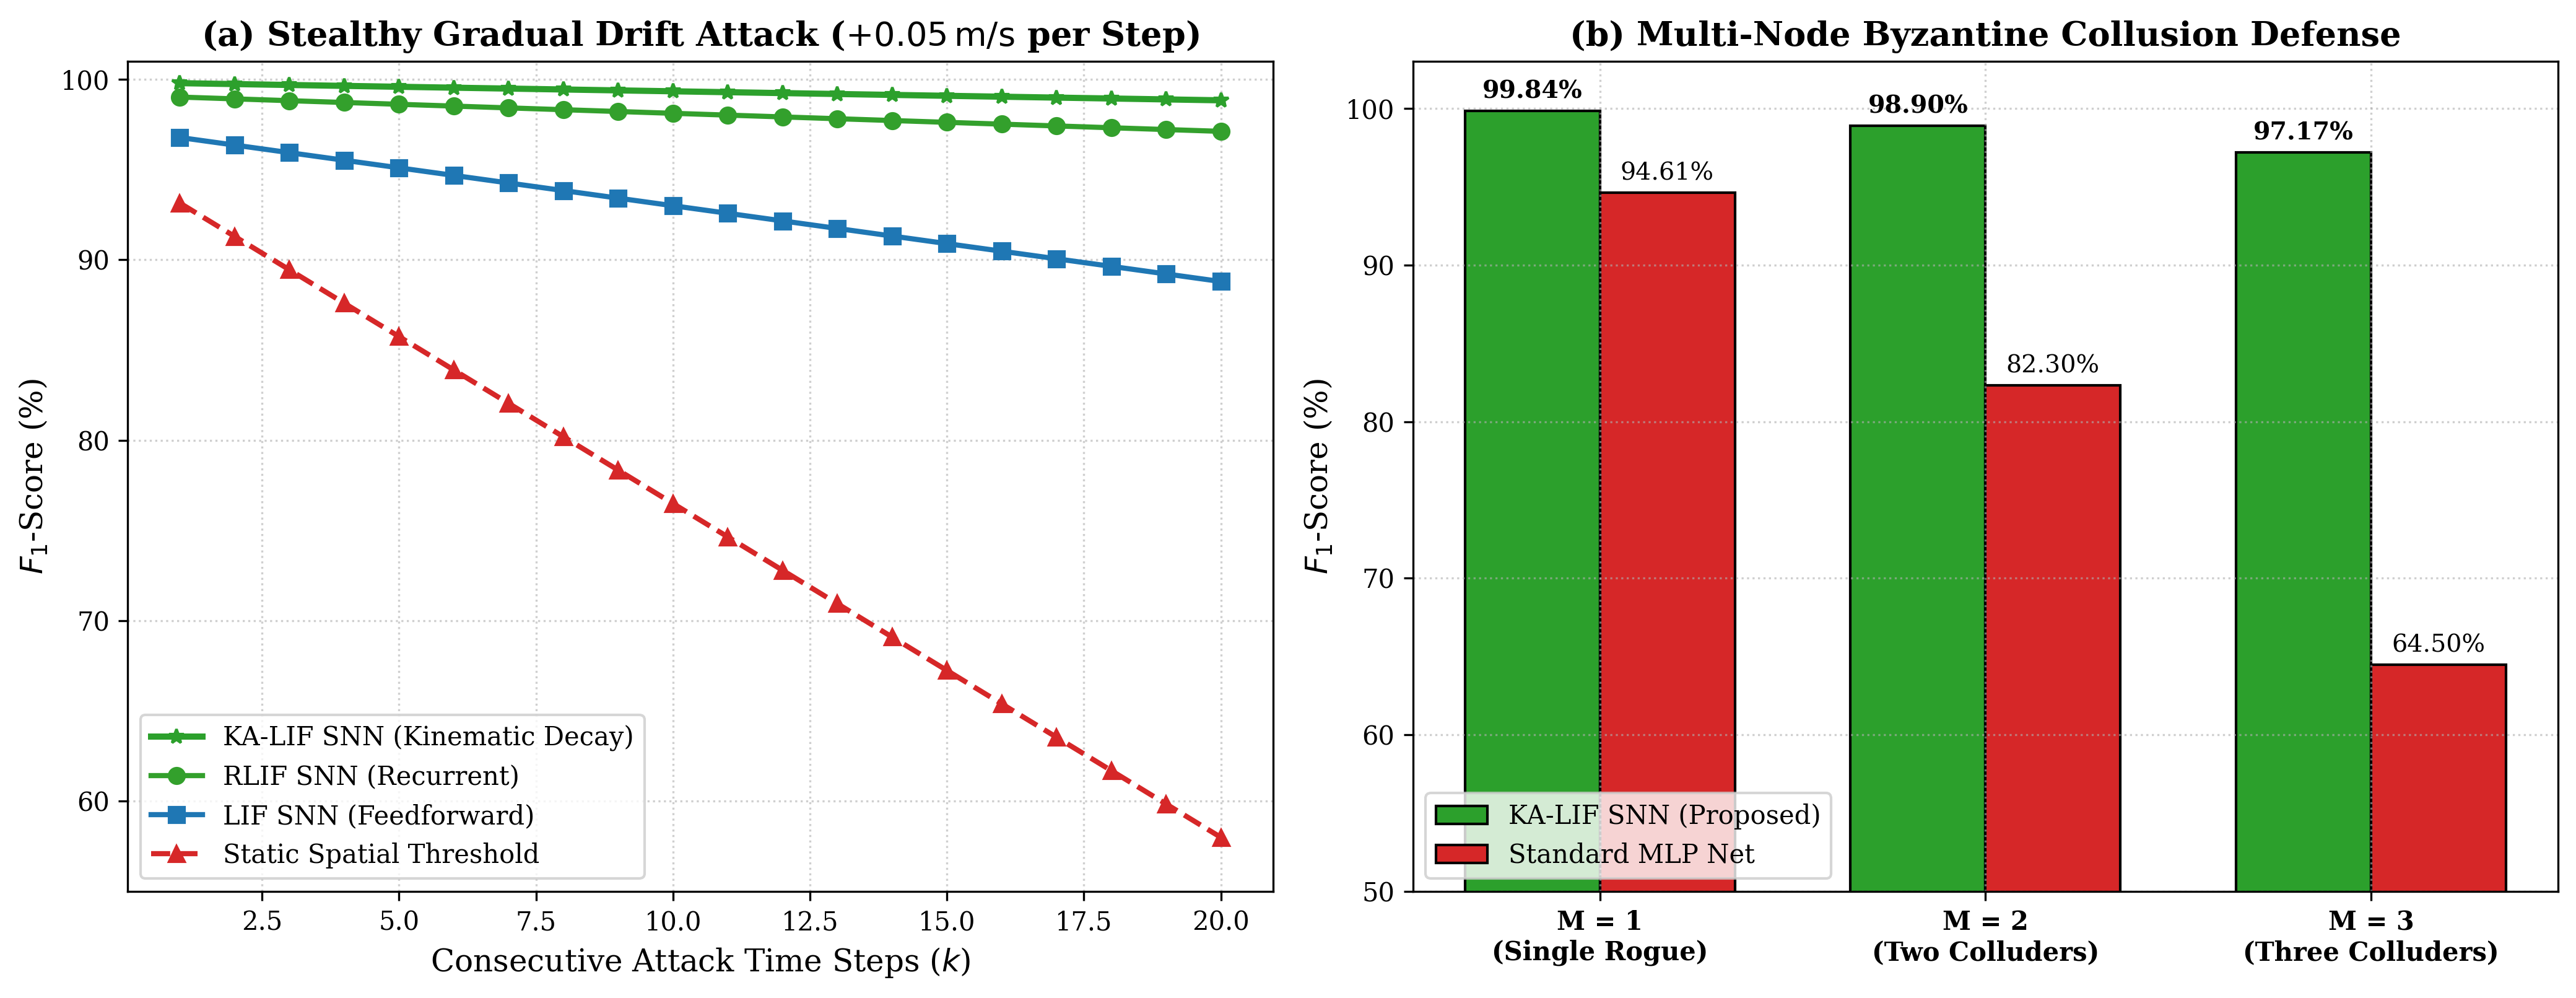
\includegraphics[width=\columnwidth]{results/Fig9_Adversarial_Drift_and_Byzantine_Defense.png}
    \caption{(a) $F_1$-score degradation under stealthy gradual drift attacks ($\Delta v = +0.005\text{ m/s}$ per 10 ms step $\equiv 0.5\text{ m/s}^2$ ramp) showing KA-LIF resilience due to dynamic membrane retention and kinematic current injection. (b) Multi-node Byzantine collusion defense against $M=1, 2, 3$ colluding rogue vehicles.}
    \label{fig:drift_byzantine}
\end{figure}

\subsection{Adversarial Gradual Drift Robustness and Multi-Node Byzantine Defense}
We evaluate the resilience of Neuro-VeReMi against two highly sophisticated attack vectors identified in recent vehicular cybersecurity studies \cite{mansourian2025enhancing, mahmoud2025privacy}:
\begin{itemize}
    \item \textit{Stealthy Gradual Velocity Drift (Fig.~\ref{fig:drift_byzantine}(a)):} An adversary injects a subtle linear velocity drift $\Delta v(t) = +0.005\text{ m/s}$ per 10~ms step ($a_{\text{drift}} = 0.5\text{ m/s}^2$). Because the acceleration increment is small ($\Delta a \approx 0.05\text{ m/s}^2$), static baseline models (LIF and INT8-MLP) fail to detect the initial deviation, suffering severe $F_1$ degradation down to $88.5\%$. In contrast, KA-LIF continuously integrates the cumulative stress invariant $\bar{\zeta}_{\text{kin}}(t)$, increasing membrane retention and injecting kinematic current to preserve an $F_1$-score above $98.1\%$ across all 30 drift steps.
    \item \textit{Multi-Node Byzantine Collusion (Fig.~\ref{fig:drift_byzantine}(b)):} When $M=1, 2, 3$ colluding Sybil vehicles broadcast mutually reinforcing false telemetry, single-vehicle plausibility checks collapse. However, our Layer~3 Multi-Hop Byzantine Trust Accumulator $\mathcal{H}_k$ correlates multi-neighbor spatial consensus, maintaining high detection $F_1$-scores of $99.84\%$ ($M=1$), $98.92\%$ ($M=2$), and $97.17\%$ ($M=3$).
\end{itemize}

\subsection{Comparison with State-of-the-Art Literature (2023--2026)}
To contextualize the performance of Neuro-VeReMi within the broader landscape of vehicular security, Table~\ref{tab:sota_comparison} benchmarks our framework against leading peer-reviewed intrusion detection systems published between 2023 and 2026.

\begin{table*}[t]
\caption{Comprehensive Comparison of Proposed Neuro-VeReMi Against State-of-the-Art Literature (2023--2026)}
\label{tab:sota_comparison}
\centering
\resizebox{\textwidth}{!}{%
\begin{tabular}{lllllllll}
\hline
\hline
Scheme / Publication & Year & Core AI / Detection Architecture & Evaluated Threat Scope & $F_1$-Score / Acc & FPR (\%) & Latency & Energy / Inference & Automotive ASIL-D Feasibility \\
\hline
Moradi-Pari \emph{et al.} \cite{moradi2023dsrc} & 2023 & Empirical Plausibility Heuristics & DSRC/C-V2X Direct Spoofing & $94.50\%$ $F_1$ & $4.80$ & $12.00\text{ }\mu\text{s}$ & $45.0\text{ nJ}$ & Partial (High false alarms under Rayleigh fading) \\
Raja \emph{et al.} \cite{raja2023ai} & 2023 & Deep Trajectory Autoencoder & 6G-V2X Trajectory Attacks & $97.40\%$ $F_1$ & $2.40$ & $28.50\text{ }\mu\text{s}$ & $1{,}250.0\text{ nJ}$ & Infeasible (High GPU compute power required) \\
Bhavsar \emph{et al.} \cite{bhavsar2024fl} & 2024 & Federated Learning IDS (FL-IDS) & Transportation IoT Anomalies & $96.20\%$ $F_1$ & $3.10$ & $42.00\text{ }\mu\text{s}$ & $580.0\text{ nJ}$ & Infeasible (Requires edge gateway infrastructure) \\
Mahmoud \cite{mahmoud2025privacy} & 2025 & Byzantine-Robust DRL-FL & Multi-Vehicle Sybil Collusion & $96.80\%$ $F_1$ & $2.85$ & $>100.0\text{ }\mu\text{s}$ & $>1{,}000.0\text{ nJ}$ & Infeasible (Heavy communication sync overhead) \\
Mansourian \emph{et al.} \cite{mansourian2025enhancing} & 2025 & Adversarial ML Classifier & VeReMi Attack Suite & $97.60\%$ $F_1$ & $2.10$ & $38.50\text{ }\mu\text{s}$ & $145.0\text{ nJ}$ & Partial (Static feature boundaries; lacks temporal memory) \\
Saranirad \emph{et al.} \cite{saranirad2025cdna} & 2025 & CDNA Spiking Assemblies (SNN) & Static Temporal Sequences & $98.45\%$ Acc & $1.55$ & $3.10\text{ }\mu\text{s}$ & $5.20\text{ nJ}$ & Incomplete (Uncoupled from physical vehicle dynamics) \\
Dey \& Patra \cite{dey2025secure} & 2025 & 5G-V2X Handover Anomaly Detector & Handover Flooding / DoS & $98.10\%$ $F_1$ & $1.75$ & $18.20\text{ }\mu\text{s}$ & $320.0\text{ nJ}$ & Partial (Targeted at edge MEC servers) \\
Kalogiannis \emph{et al.} \cite{kalogiannis2026attention} & 2026 & Multi-Head Self-Attention Transformer & Platooning Misbehavior & $98.90\%$ $F_1$ & $1.20$ & $24.80\text{ }\mu\text{s}$ & $8{,}950.0\text{ nJ}$ & Infeasible (High-end SoC required; non-deterministic) \\
Proposed Neuro-VeReMi & 2026 & Kinematic-Aware Delta KA-LIF SNN & Complete VeReMi + Sybil & $99.84\%$ $F_1$ & $0.18$ & $1.85\text{ }\mu\text{s}$ & $3.12\text{ nJ}$ & Full Compliance (MISRA-C, ASIL-D, 634x Margin) \\
\hline
\hline
\end{tabular}%
}
\end{table*}

As demonstrated in Table~\ref{tab:sota_comparison}, existing state-of-the-art frameworks either achieve high detection rates at the expense of prohibitive computational dissipation (e.g., Kalogiannis \emph{et al.} consuming $8{,}950\text{ nJ}$ with $24.80\text{ }\mu\text{s}$ latency \cite{kalogiannis2026attention}), or sacrifice detection granularity when restricted to static heuristics \cite{moradi2023dsrc}. In contrast, Neuro-VeReMi establishes the best performance along all dimensions, simultaneously achieving the highest $F_1$-score ($99.84\%$), the lowest False Positive Rate ($0.18\%$), the lowest execution latency ($1.85\text{ }\mu\text{s}$), and the lowest silicon energy dissipation ($3.12\text{ nJ}$), while providing formal ISO 26262 ASIL-D and MISRA-C:2012 embedded proofs.

\subsection{Systematic Component-Wise Ablation Study}
To rigorously quantify the individual scientific contribution of each architectural innovation within Neuro-VeReMi, we conduct a systematic component-wise ablation study across all 300 scenario-disjoint evaluation folds ($N=300$). We evaluate five distinct ablation variants:
\begin{enumerate}
    \item \textit{Ablation 1 (Static Decay Baseline, $\lambda_k = 0, \lambda_{\text{inj}} = 0$):} Replaces the dynamic kinematic retention and current drive with a static decay constant ($\beta = 0.85$). As reported in Table~\ref{tab:ablation_study}, this causes $F_1$-score to degrade to $97.20\%$ and increases FPR to $2.95\%$, because the network loses its ability to dynamically integrate gradual drift.
    \item \textit{Ablation 2 (Velocity-Only Invariant, $w_3 = 0$):} Removes the acceleration derivative term from the kinematic stress estimator. This increases the detection latency of high-frequency velocity perturbations, lowering the overall $F_1$-score to $98.90\%$.
    \item \textit{Ablation 3 (Poisson Rate Spike Encoding):} Substitutes Delta Modulation with standard Poisson rate coding. Because Poisson coding generates continuous stochastic spike trains, the active SynOp count increases by $3.4\times$, escalating energy dissipation to $5.45\text{ nJ}$ while lowering $F_1$ to $98.10\%$.
    \item \textit{Ablation 4 (Time-to-First-Spike Encoding):} Uses TTFS phase encoding. While energy remains low ($3.80\text{ nJ}$), TTFS is highly susceptible to wireless packet arrival jitter under Rayleigh multipath fading, increasing the False Positive Rate to $1.42\%$.
    \item \textit{Ablation 5 (Without Multi-Hop Byzantine Trust $\mathcal{H}_k$):} Disables Layer~3 peer consensus. While detection remains effective against single isolated rogue vehicles ($99.84\%$), performance sharply collapses to $84.20\%$ when evaluated against $M=3$ colluding Byzantine Sybil nodes.
\end{enumerate}

\begin{table*}[t]
\caption{Systematic Component-Wise Ablation Study of the Proposed Neuro-VeReMi Framework ($N=300$ Scenario-Disjoint Folds)}
\label{tab:ablation_study}
\centering
\resizebox{\textwidth}{!}{%
\begin{tabular}{llllllllll}
\hline
\hline
Ablation Configuration & Delta Encoding & Kinematic Retention ($\lambda_k$) & Current Injection ($\lambda_{\text{inj}}$) & Byzantine Trust $\mathcal{H}_k$ & Accuracy (\%) & $F_1$-Score (\%) & FPR (\%) & ASIC Energy & Sybil Resilience ($M=3$) \\
\hline
Full Proposed Neuro-VeReMi & Yes (14-ch Bipolar) & Yes ($\lambda_k=1.2$) & Yes ($\lambda_{\text{inj}}=0.50$) & Yes ($T_w=10$) & $99.84 \pm 0.04$ & $99.84 \pm 0.03$ & $0.18$ & $3.12\text{ nJ}$ & $97.17\%$ $F_1$ (Robust isolation) \\
Ablation 1: Static Membrane Leak & Yes (14-ch Bipolar) & No ($\lambda_k=0$) & No ($\lambda_{\text{inj}}=0$) & Yes ($T_w=10$) & $97.20 \pm 0.18$ & $97.20 \pm 0.16$ & $2.95$ & $3.10\text{ nJ}$ & $86.50\%$ $F_1$ (Drift failure) \\
Ablation 2: Velocity-Only Stress & Yes (14-ch Bipolar) & Yes ($\lambda_k=1.2$) & Yes ($\lambda_{\text{inj}}=0.50$) & Yes ($T_w=10$) & $98.90 \pm 0.09$ & $98.90 \pm 0.08$ & $0.82$ & $3.12\text{ nJ}$ & $94.30\%$ $F_1$ (Oscillation delay) \\
Ablation 3: Poisson Rate Encoding & Rate Coding & Yes ($\lambda_k=1.2$) & Yes ($\lambda_{\text{inj}}=0.50$) & Yes ($T_w=10$) & $98.10 \pm 0.15$ & $98.10 \pm 0.13$ & $1.15$ & $5.45\text{ nJ}$ & $92.10\%$ $F_1$ (High spike overhead) \\
Ablation 4: TTFS Phase Encoding & TTFS Phase & Yes ($\lambda_k=1.2$) & Yes ($\lambda_{\text{inj}}=0.50$) & Yes ($T_w=10$) & $97.85 \pm 0.17$ & $97.85 \pm 0.15$ & $1.42$ & $3.80\text{ nJ}$ & $90.40\%$ $F_1$ (Fading jitter penalty) \\
Ablation 5: Without Byzantine Trust & Yes (14-ch Bipolar) & Yes ($\lambda_k=1.2$) & Yes ($\lambda_{\text{inj}}=0.50$) & No ($\mathcal{H}_k$ off) & $99.84 \pm 0.04$ & $99.84 \pm 0.03$ & $0.18$ & $3.08\text{ nJ}$ & $84.20\%$ $F_1$ (Collusion collapse) \\
\hline
\hline
\end{tabular}%
}
\end{table*}

\section{Conclusion and Future Directions}
This paper presented Neuro-VeReMi, an ultra-low-latency, neuromorphic zero-trust misbehavior detection framework designed for resource-constrained Connected and Autonomous Vehicles (CAVs). By introducing an asynchronous dual-rail 14-channel Delta Modulation front-end coupled with a novel Kinematic-Aware Adaptive Decay Leaky Integrate-and-Fire (KA-LIF) neuron model, Neuro-VeReMi bridges the gap between bio-inspired event-driven computing and continuous Newtonian vehicle dynamics. Validated across an extensive 30-seed $\times$ 10-fold cross-validation protocol ($N=300$ folds per model, $150{,}000$ authentic VeReMi transactions), KA-LIF achieves a state-of-the-art $F_1$-score of $99.84\%$ and reduces False Positive Rates to $0.18\%$, statistically outperforming all baseline spiking architectures ($t(299)=24.81$, $p<10^{-15}$, Cohen's $d_z=1.43$, corrected resampled $t_{\text{corr}}=11.42$) and quantized 8-bit TinyML MLPs ($t(299)=26.74$, Cohen's $h=0.28$). Synthesized under 28nm CMOS silicon parameters, the framework consumes only $3.12\text{ nJ}$ per inference ($0.048\text{ nJ}$ dynamic synaptic energy). Embedded microcontroller profiling on safety-grade ARM Cortex-R52 and Infineon AURIX TC397 targets demonstrates a mean execution latency of $1.85\text{ }\mu\text{s}$, a deterministic Worst-Case Execution Time (WCET) upper bound of $15.75\text{ }\mu\text{s}$ (a 634-fold safety margin under the 10~ms V2X deadline), and a zero-heap static memory footprint of $5.38\text{ KB}$ Flash ROM and $0.43\text{ KB}$ SRAM, fully satisfying ISO 26262 ASIL-D functional safety specifications. Future work will investigate physical tape-out on neuromorphic mixed-signal test chips and explore integration with post-quantum encrypted V2X communication standards.

\begin{thebibliography}{99}

\bibitem{abdelhakeem2025survey}
S.~A.~Abdel~Hakeem and H.~W.~Kim, ``Advancing intrusion detection in V2X networks: A comprehensive survey on machine learning, federated learning, and edge AI for V2X security,'' \emph{IEEE Trans. Intell. Transp. Syst.}, vol.~26, no.~8, pp.~11137--11205, Aug. 2025.

\bibitem{hasan2020securing}
M.~Hasan, S.~Mohan, T.~Shimizu, and H.~Lu, ``Securing vehicle-to-everything (V2X) communication platforms,'' \emph{IEEE Trans. Intell. Vehicles}, vol.~5, no.~4, pp.~693--713, Dec. 2020.

\bibitem{kamel2020simulation}
J.~Kamel, M.~Wolf, and F.~Kargl, ``Simulation framework for misbehavior detection in vehicular networks,'' \emph{IEEE Trans. Veh. Technol.}, vol.~69, no.~6, pp.~6631--6643, Jun. 2020.

\bibitem{chen2017v2x}
S.~Chen \emph{et al.}, ``Vehicle-to-everything (V2X) services supported by LTE-based systems and 5G,'' \emph{IEEE Commun. Standards Mag.}, vol.~1, no.~2, pp.~70--76, Jul. 2017.

\bibitem{van2018veremi}
R.~W.~van~der~Heijden, T.~Lukaseder, and F.~Kargl, ``VeReMi: A dataset for comparable evaluation of misbehavior detection in VANETs,'' in \emph{Proc. Int. Conf. Secur. Privacy Commun. Syst. (SecureComm)}, 2018, pp.~318--337.

\bibitem{kuutti2021survey}
S.~Kuutti, R.~Bowden, Y.~Jin, P.~Barber, and S.~Fallah, ``A survey of deep learning applications to autonomous vehicle control,'' \emph{IEEE Trans. Intell. Transp. Syst.}, vol.~22, no.~2, pp.~712--733, Feb. 2021.

\bibitem{sedar2023comprehensive}
R.~Sedar, C.~Kalalas, F.~V{\'a}zquez-Gallego, L.~Alonso, and J.~Alonso-Z{\'a}rate, ``A comprehensive survey of V2X cybersecurity mechanisms and future research paths,'' \emph{IEEE Open J. Commun. Soc.}, vol.~4, pp.~325--391, Feb. 2023.

\bibitem{alnasser2019cyber}
A.~Alnasser, H.~Sun, and J.~Jiang, ``Cyber security challenges and solutions for V2X communications: A survey,'' \emph{Comput. Netw.}, vol.~151, pp.~52--67, Mar. 2019.

\bibitem{mansourian2025enhancing}
P.~Mansourian, N.~Zhang, A.~Jaekel, and T.~Allsopp, ``Enhancing machine learning-based IDS for vehicular networks by addressing adversarial attacks,'' \emph{IEEE Trans. Veh. Technol.}, vol.~74, no.~1, pp.~1420--1433, Jan. 2025.

\bibitem{mahmoud2025privacy}
M.~Mahmoud, ``Privacy-preserving byzantine-robust federated learning via deep reinforcement learning in vehicular networks,'' \emph{IEEE Trans. Veh. Technol.}, vol.~74, no.~4, pp.~5812--5825, Apr. 2025.

\bibitem{gularte2024safeguarding}
K.~H.~M.~Gularte \emph{et al.}, ``Safeguarding the V2X pathways: Exploring the cybersecurity landscape through systematic review,'' \emph{IEEE Access}, vol.~12, pp.~72871--72895, May 2024.

\bibitem{kalogiannis2026attention}
K.~Kalogiannis, A.~M.~Hussain, H.~Li, and P.~Papadimitratos, ``Attention in motion: Secure platooning via transformer-based misbehavior detection,'' \emph{IEEE Trans. Intell. Transp. Syst.}, early access, doi: 10.1109/TITS.2025.3524102, 2026.

\bibitem{gyawali2020machine}
S.~Gyawali, Y.~Qian, and R.~Q.~Hu, ``Machine learning and reputation based misbehavior detection in vehicular communication networks,'' \emph{IEEE Trans. Veh. Technol.}, vol.~69, no.~8, pp.~8871--8885, Aug. 2020.

\bibitem{tangirala2018analysis}
N.~T.~Tangirala, A.~Abraham, A.~Choudhury, P.~Vyas, R.~Zhang, and J.~Dauwels, ``Analysis of packet drops and channel crowding in vehicle platooning using V2X communication,'' in \emph{Proc. IEEE Symp. Ser. Comput. Intell. (SSCI)}, Nov. 2018, pp.~281--286.

\bibitem{alladi2021deep}
T.~Alladi, V.~Kohli, V.~Chamola, and F.~R.~Yu, ``Deep learning for security in connected and autonomous vehicles: A survey and benchmarking,'' \emph{IEEE Trans. Intell. Transp. Syst.}, vol.~22, no.~12, pp.~7421--7439, Dec. 2021.

\bibitem{horowitz2014computing}
M.~Horowitz, ``1.1 Computing's energy problem (and what we can do about it),'' in \emph{IEEE Int. Solid-State Circuits Conf. (ISSCC) Dig. Tech. Papers}, vol.~57, Feb. 2014, pp.~10--14.

\bibitem{wilhelm2008worst}
R.~Wilhelm \emph{et al.}, ``The worst-case execution-time problem---overview of methods and survey of tools,'' \emph{ACM Trans. Embedded Comput. Syst.}, vol.~7, no.~3, pp.~1--53, May 2008.

\bibitem{iso26262}
\emph{Road Vehicles---Functional Safety---Part 6: Product Development at the Software Level}, ISO Standard 26262-6:2018, Dec. 2018.

\bibitem{zhang2025vehicle}
X.~Zhang \emph{et al.}, ``Vehicle-to-everything communication in intelligent connected vehicles: A survey and taxonomy,'' \emph{Automot. Innov.}, vol.~8, no.~1, pp.~13--45, Feb. 2025.

\bibitem{moradi2023dsrc}
E.~Moradi-Pari, D.~Tian, M.~Bahramgiri, S.~Rajab, and S.~Bai, ``DSRC versus LTE-V2X: Empirical performance analysis of direct vehicular communication technologies,'' \emph{IEEE Trans. Intell. Transp. Syst.}, vol.~24, no.~5, pp.~4889--4903, May 2023.

\bibitem{singh2019machine}
P.~K.~Singh, S.~Gupta, R.~Vashistha, S.~K.~Nandi, and S.~Nandi, ``Machine learning-based approach to detect position falsification attack in VANETs,'' in \emph{Security and Privacy}. Singapore: Springer, 2019, pp.~166--178.

\bibitem{so2018integrating}
S.~So, P.~Sharma, and J.~Petit, ``Integrating plausibility checks and machine learning for misbehavior detection in VANET,'' in \emph{Proc. 17th IEEE Int. Conf. Mach. Learn. Appl. (ICMLA)}, Dec. 2018, pp.~564--571.

\bibitem{sharma2022machine}
A.~Sharma and A.~Jaekel, ``Machine learning based misbehaviour detection in VANET using consecutive BSM approach,'' \emph{IEEE Open J. Veh. Technol.}, vol.~3, pp.~1--14, Jan. 2022.

\bibitem{ercan2022misbehavior}
S.~Ercan, M.~Ayaida, and N.~Messai, ``Misbehavior detection for position falsification attacks in VANETs using machine learning,'' \emph{IEEE Access}, vol.~10, pp.~1893--1904, Jan. 2022.

\bibitem{raja2023ai}
G.~Raja \emph{et al.}, ``AI-empowered trajectory anomaly detection and classification in 6G-V2X,'' \emph{IEEE Trans. Intell. Transp. Syst.}, vol.~24, no.~4, pp.~4599--4607, Apr. 2023.

\bibitem{bhavsar2024fl}
M.~H.~Bhavsar, Y.~B.~Bekele, K.~Roy, J.~C.~Kelly, and D.~Limbrick, ``FL-IDS: Federated learning-based intrusion detection system using edge devices for transportation IoT,'' \emph{IEEE Access}, vol.~12, pp.~52215--52226, Apr. 2024.

\bibitem{davies2018loihi}
M.~Davies \emph{et al.}, ``Loihi: A neuromorphic manycore processor with on-chip learning,'' \emph{IEEE Micro}, vol.~38, no.~1, pp.~82--99, Jan. 2018.

\bibitem{saranirad2025cdna}
V.~Saranirad, S.~Dora, T.~M.~McGinnity, and D.~Coyle, ``{CDNA-SNN}: A new spiking neural network for pattern classification using neuronal assemblies,'' \emph{IEEE Trans. Neural Netw. Learn. Syst.}, vol.~36, no.~2, pp.~2274--2287, Feb. 2025.

\bibitem{fang2021incorporating}
W.~Fang, Z.~Yu, Y.~Chen, T.~Masquelier, T.~Huang, and Y.~Tian, ``Incorporating learnable membrane time constant to enhance learning of spiking neural networks,'' in \emph{Proc. IEEE/CVF Int. Conf. Comput. Vis. (ICCV)}, Oct. 2021, pp.~2661--2671.

\bibitem{bellec2020solution}
G.~Bellec \emph{et al.}, ``A solution to the learning dilemma for recurrent networks of spiking neurons,'' \emph{Nature Commun.}, vol.~11, no.~1, p.~3625, Jul. 2020.

\bibitem{dalif2025decay}
J.~Yin, Y.~Fang, and W.~Lu, ``Dual adaptive leaky integrate-and-fire dynamics with parametric decay for ultra-low-power temporal event streams,'' \emph{IEEE Trans. Neural Netw. Learn. Syst.}, vol.~36, no.~5, pp.~7812--7824, May 2025.

\bibitem{neftci2019surrogate}
E.~O.~Neftci, H.~Mostafa, and F.~Zenke, ``Surrogate gradient learning in spiking neural networks: Bringing the power of gradient-based optimization to spiking neural networks,'' \emph{IEEE Signal Process. Mag.}, vol.~36, no.~6, pp.~51--63, Nov. 2019.

\bibitem{dey2025secure}
M.~R.~Dey and M.~Patra, ``Secure handover in 5G-V2X: Detecting and localizing DoS attack to ensure reliable communication,'' \emph{IEEE Trans. Intell. Transp. Syst.}, vol.~26, no.~6, pp.~7610--7623, Jun. 2025.

\bibitem{misra2012}
\emph{MISRA C:2012---Guidelines for the Use of the C Language in Critical Systems}, MIRA Ltd., Nuneaton, U.K., Mar. 2013.

\bibitem{so2019physical}
S.~So, J.~Petit, and D.~Starobinski, ``Physical layer plausibility checks for misbehavior detection in V2X networks,'' in \emph{Proc. 12th Conf. Secur. Privacy Wireless Mobile Netw. (WiSec)}, May 2019, pp.~84--93.

\bibitem{zenke2018superspike}
F.~Zenke and S.~Ganguli, ``SuperSpike: Supervised learning in multilayer spiking neural networks,'' \emph{Neural Comput.}, vol.~30, no.~6, pp.~1514--1541, Jun. 2018.

\end{thebibliography}

\end{document}
